\documentclass[11pt,a4paper]{article}
\usepackage[utf8]{inputenc}
\usepackage{amsmath}
\usepackage{amsfonts}
\usepackage{amssymb}
\usepackage{graphicx}
\usepackage{geometry}
\usepackage{fancyhdr}
\usepackage{hyperref}
\usepackage{bm}
\usepackage{array}
\usepackage{booktabs}
\usepackage{tikz}
\usepackage{pgfplots}
\usepackage{algorithm}
\usepackage{algorithmic}
\usepackage{subfig}
\usepackage{multirow}
\usepackage{color}
\usepackage{xcolor}

\geometry{margin=1in}
\pagestyle{fancy}
\fancyhf{}
\rhead{Singularity Analysis Equations}
\lhead{Hybrid Serial-Cable Driven Robot}
\cfoot{\thepage}

\title{Mathematical Equations for Singularity Analysis of \\
Hybrid Serial-Cable Driven Planar Robot}
\author{Implementation Reference Document}
\date{\today}

\begin{document}

\maketitle

\tableofcontents
\newpage

\section{Robot Configuration and Parameters}

\subsection{System Description}
The hybrid serial-cable driven planar robot combines a serial manipulator with cable actuation. The system comprises:

\begin{itemize}
    \item A 2-DOF serial kinematic chain (links connected by revolute joints)
    \item Two cables both attached to the end-effector point M
    \item Fixed cable anchor points at positions $(-L, 0)$ and $(L, 0)$
    \item Cable actuation providing additional forces and constraints at point M
    \item Hybrid actuation: joint motors + cable tensions
\end{itemize}

\textbf{Key Characteristics:}
\begin{itemize}
    \item The serial chain provides the primary positioning mechanism
    \item Cables apply forces directly to the end-effector point M
    \item Cable lengths vary as the serial chain moves
    \item Cable tensions can assist or modify the motion capabilities
    \item System redundancy allows for singularity avoidance
\end{itemize}

\begin{figure}[h]
\centering
% TikZ diagram for the hybrid serial-cable driven robot
% Cable angles α₁ and α₂ are computed using atan2 for robust quadrant handling
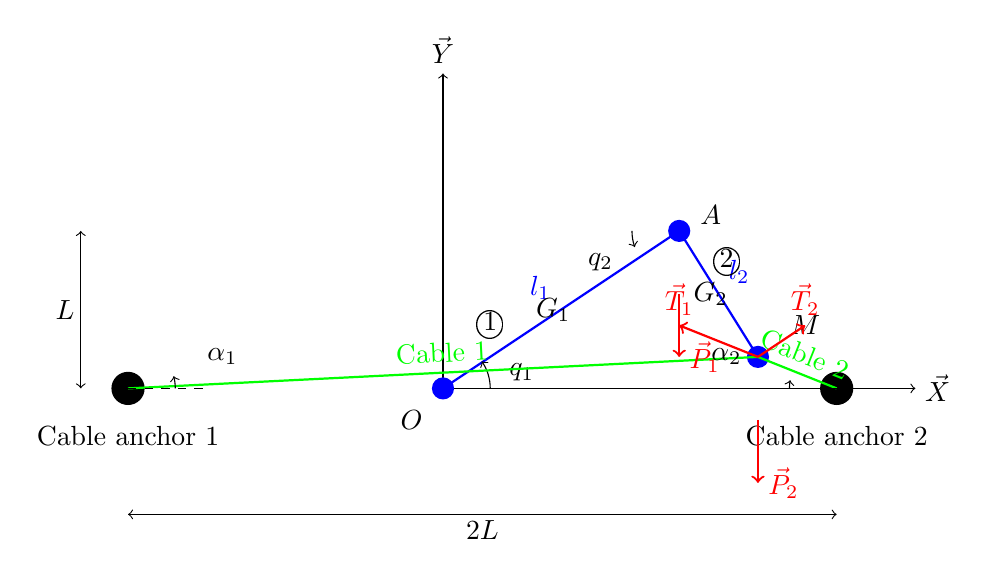
\begin{tikzpicture}[scale=2]
    % Coordinate system
    \draw[->] (0,0) -- (3,0) node[right] {$\vec{X}$};
    \draw[->] (0,0) -- (0,2) node[above] {$\vec{Y}$};
    \node at (-0.2,-0.2) {$O$};
    
    % Fixed base points
    \fill[black] (-2,0) circle (3pt);
    \fill[black] (2.5,0) circle (3pt);
    \node at (-2,-0.3) {Cable anchor 1};
    \node at (2.5,-0.3) {Cable anchor 2};
    
    % Serial arm links
    \draw[thick, blue] (0,0) -- (1.5,1) node[midway, above left] {$l_1$};
    \draw[thick, blue] (1.5,1) -- (2,0.2) node[midway, above right] {$l_2$};
    
    % Joints
    \fill[blue] (0,0) circle (2pt);
    \fill[blue] (1.5,1) circle (2pt);
    \fill[blue] (2,0.2) circle (2pt);
    
    % Joint labels
    \node at (0.3,0.4) {\textcircled{1}};
    \node at (1.8,0.8) {\textcircled{2}};
    \node at (2.3,0.4) {$M$};
    
    % Joint angles
    \draw[->] (0.3,0) arc (0:35:0.3);
    \node at (0.5,0.1) {$q_1$};
    \draw[->] (1.2,1) arc (180:200:0.3);
    \node at (1.0,0.8) {$q_2$};
    
    % Cable lines (both connected to end-effector M)
    \draw[green, thick] (-2,0) -- (2,0.2) node[midway, above, sloped] {Cable 1};
    \draw[green, thick] (2.5,0) -- (2,0.2) node[midway, above, sloped] {Cable 2};
    
    % Cable angles
    \draw[dashed] (-2,0) -- (-1.5,0);
    \draw[->] (-1.7,0) arc (0:15:0.3);
    \node at (-1.4,0.2) {$\alpha_1$};
    
    \draw[dashed] (2.5,0) -- (2,0);
    \draw[->] (2.2,0) arc (180:170:0.3);
    \node at (1.8,0.2) {$\alpha_2$};
    
    % Forces and positions
    \draw[->, red, thick] (1.5,0.6) -- (1.5,0.2) node[right] {$\vec{P}_1$};
    \draw[->, red, thick] (2,-0.2) -- (2,-0.6) node[right] {$\vec{P}_2$};
    
    % Cable tensions (both acting on point M)
    \draw[->, red, thick] (2,0.2) -- (1.5,0.4) node[above] {$\vec{T}_1$};
    \draw[->, red, thick] (2,0.2) -- (2.3,0.4) node[above] {$\vec{T}_2$};
    
    % Dimensions
    \draw[<->] (-2,-0.8) -- (2.5,-0.8);
    \node at (0.25,-0.9) {$2L$};
    \draw[<->] (-2.3,0) -- (-2.3,1);
    \node at (-2.4,0.5) {$L$};
    
    % Points G1, G2, A
    \node at (0.7,0.5) {$G_1$};
    \node at (1.7,0.6) {$G_2$};
    \node at (1.7,1.1) {$A$};
\end{tikzpicture}
\caption{Schematic of the hybrid serial-cable driven planar robot. Cable angles $\alpha_1$ and $\alpha_2$ are computed using $\text{atan2}$ for robust quadrant handling.}
\label{fig:robot_config}
\end{figure}

The hybrid configuration provides:
\begin{enumerate}
    \item Extended workspace through serial chain reach
    \item Enhanced stiffness and precision via cable pre-tensioning  
    \item Singularity avoidance through redundant actuation
    \item Improved dynamic performance with distributed actuation
\end{enumerate}

\subsection{Specific Robot Configuration}
Based on the schematic in Figure \ref{fig:robot_config}, the robot has the following characteristics:

\subsubsection{Serial Chain}
\begin{itemize}
    \item Two revolute joints with angles $q_1$ and $q_2$
    \item Link lengths: $l_1$ and $l_2$  
    \item Joint centers at $O$ (base), $A$ (elbow), and $M$ (end-effector)
    \item Centers of mass at $G_1$ and $G_2$
\end{itemize}

\subsubsection{Cable System}
\begin{itemize}
    \item Two cables attached to the end-effector point M
    \item Fixed cable anchor points positioned at $(-L, 0)$ and $(L, 0)$ 
    \item Both cables connect from their respective anchor points to point M
    \item Cable tensions $T_1$ and $T_2$ act directly on the end-effector
    \item Cable angles $\alpha_1$ and $\alpha_2$ measured from horizontal to cable directions
\end{itemize}

\subsubsection{Force System}  
\begin{itemize}
    \item Gravitational forces $P_1$ and $P_2$ acting at centers of mass $G_1$ and $G_2$
    \item Cable tensions $T_1$ and $T_2$ both acting at end-effector point M
    \item Cable forces act along the directions from M to respective anchor points
    \item Joint torques from serial actuators (if present)
    \item Net force equilibrium at point M from both cable tensions
\end{itemize}

\subsubsection{Cable Force Vectors}
The cable tension forces acting on the end-effector are:
\begin{align}
\bm{F}_1 &= T_1 \bm{u}_1 = T_1 \frac{\bm{A}_1 - \bm{p}_M}{\rho_1} = -T_1 \frac{\bm{p}_M - \bm{A}_1}{\rho_1} \\
\bm{F}_2 &= T_2 \bm{u}_2 = T_2 \frac{\bm{A}_2 - \bm{p}_M}{\rho_2} = -T_2 \frac{\bm{p}_M - \bm{A}_2}{\rho_2}
\end{align}

The total cable force on the end-effector is:
\begin{align}
\bm{F}_{cable} &= \bm{F}_1 + \bm{F}_2 \\
&= -T_1 \frac{1}{\rho_1}\begin{bmatrix} x_M + L \\ y_M \end{bmatrix} - T_2 \frac{1}{\rho_2}\begin{bmatrix} x_M - L \\ y_M \end{bmatrix}
\end{align}

\subsection{Robot Parameters}
For the specific configuration shown in Figure \ref{fig:robot_config}:
\begin{align}
n_j &= 2 \quad \text{(number of serial joints)} \\
n_c &= 2 \quad \text{(number of cables)} \\
n_{dof} &= 2 \quad \text{(planar positioning: } x, y \text{)} \\
l_1, l_2 &= \text{link lengths of serial chain} \\
L &= \text{half-span of cable anchor points} \\
m_1, m_2 &= \text{masses of links 1 and 2} \\
I_1, I_2 &= \text{moments of inertia about centers of mass}
\end{align}

\subsubsection{Geometric Parameters}
\begin{align}
\text{Base frame origin: } &\quad O = (0, 0) \\
\text{Cable anchor points: } &\quad A_1 = (-L, 0), \quad A_2 = (L, 0) \\
\text{Joint 1 position: } &\quad \text{at origin } O \\
\text{Joint 2 position: } &\quad A = (l_1 \cos q_1, l_1 \sin q_1) \\
\text{End-effector position: } &\quad M = A + (l_2 \cos(q_1 + q_2), l_2 \sin(q_1 + q_2))
\end{align}

\subsubsection{Cable Geometry}
\begin{align}
\text{Cable 1 length: } &\quad \rho_1 = \|M - A_1\| \\
\text{Cable 2 length: } &\quad \rho_2 = \|M - A_2\| \\
\text{Cable 1 angle: } &\quad \alpha_1 = \text{atan2}(y_M, x_M + L) \\
\text{Cable 2 angle: } &\quad \alpha_2 = \text{atan2}(y_M, x_M - L)
\end{align}

\subsection{Coordinate Systems}
The robot coordinate systems are defined as follows:
\begin{align}
\{O\} &: \text{base frame (fixed world frame)} \\
\{E\} &: \text{end-effector frame (moving frame)} \\
\{C_i\} &: \text{cable attachment frame } i, \quad i = 1, 2, \ldots, n_c \\
\{J_j\} &: \text{joint frame } j, \quad j = 1, 2, \ldots, n_j
\end{align}

\subsubsection{Transformation Matrices}
Homogeneous transformation matrices provide a unified framework for representing both rotation and translation in robotics. For the hybrid serial-cable driven planar robot, these transformations are essential for relating different coordinate frames.

\textbf{General Homogeneous Transformation:}
The homogeneous transformation from frame $\{i\}$ to frame $\{j\}$ is:
\begin{align}
\bm{T}_j^i &= \begin{bmatrix}
\bm{R}_j^i & \bm{p}_j^i \\
\bm{0}^T & 1
\end{bmatrix}
\end{align}

Where:
\begin{itemize}
    \item $\bm{R}_j^i \in SO(2)$: rotation matrix from frame $\{i\}$ to frame $\{j\}$
    \item $\bm{p}_j^i \in \mathbb{R}^2$: position vector of origin of frame $\{j\}$ expressed in frame $\{i\}$
    \item $\bm{0}^T = [0 \quad 0]$: zero row vector
\end{itemize}

\textbf{2D Planar Transformation:}
For planar motion, the transformation matrix becomes:
\begin{align}
\bm{T}_j^i &= \begin{bmatrix}
\cos\theta_{ij} & -\sin\theta_{ij} & x_{ij} \\
\sin\theta_{ij} & \cos\theta_{ij} & y_{ij} \\
0 & 0 & 1
\end{bmatrix}
\end{align}

Where:
\begin{align}
\theta_{ij} &: \text{rotation angle from frame } \{i\} \text{ to frame } \{j\} \\
x_{ij}, y_{ij} &: \text{translation components from frame } \{i\} \text{ to frame } \{j\}
\end{align}

\textbf{Properties of Transformation Matrices:}
\begin{enumerate}
    \item \textbf{Composition:} $\bm{T}_k^i = \bm{T}_j^i \bm{T}_k^j$
    \item \textbf{Inverse:} $(\bm{T}_j^i)^{-1} = \bm{T}_i^j = \begin{bmatrix} (\bm{R}_j^i)^T & -(\bm{R}_j^i)^T \bm{p}_j^i \\ \bm{0}^T & 1 \end{bmatrix}$
    \item \textbf{Identity:} $\bm{T}_i^i = \bm{I}_3$
    \item \textbf{Determinant:} $\det(\bm{T}_j^i) = 1$
\end{enumerate}

\textbf{Derivation Methodology: Step-by-Step Approach}

To systematically derive transformation matrices, follow this structured approach:

\textbf{General Derivation Steps:}
\begin{enumerate}
    \item \textbf{Frame Assignment}: Clearly define coordinate frames with their origins and orientations
    \item \textbf{Geometric Analysis}: Identify translation and rotation relationships between frames
    \item \textbf{Parameter Extraction}: Extract angle $\theta$ and translation components $(x, y)$
    \item \textbf{Matrix Construction}: Build the transformation matrix using the standard form
    \item \textbf{Verification}: Check results using geometric reasoning or known points
\end{enumerate}

\textbf{Use Case Exercise: Mobile Robot Navigation}

\textbf{Problem Statement:}
A mobile robot starts at the origin of a world frame $\{W\}$. The robot first translates 3 units along the positive $x$-axis, then rotates $45^{\circ}$ counterclockwise, and finally translates 2 units along its new local $x$-axis direction. Find the complete transformation matrix from the world frame to the robot's final frame $\{R\}$.

\begin{figure}[htbp]
\centering
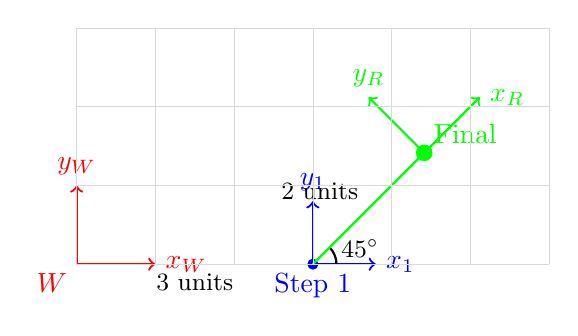
\begin{tikzpicture}[scale=1.0]
    % World frame
    \draw[thick, ->, red] (0,0) -- (1,0) node[right] {$x_W$};
    \draw[thick, ->, red] (0,0) -- (0,1) node[above] {$y_W$};
    \node[below left, red] at (0,0) {$W$};
    
    % Step 1: Translation
    \draw[dashed, blue] (0,0) -- (3,0);
    \fill[blue] (3,0) circle (2pt);
    \node[below, blue] at (3,0) {Step 1};
    \draw[thick, ->, blue] (3,0) -- (3.8,0) node[right] {$x_1$};
    \draw[thick, ->, blue] (3,0) -- (3,0.8) node[above] {$y_1$};
    
    % Step 2: Rotation (45 degrees)
    \draw[thick] (3.3,0) arc (0:45:0.3);
    \node at (3.6,0.2) {\small $45^{\circ}$};
    
    % Step 3: Final position
    \draw[thick, green] (3,0) -- (3+2*0.707, 2*0.707);
    \fill[green] (3+2*0.707, 2*0.707) circle (3pt);
    \node[above right, green] at (3+2*0.707, 2*0.707) {Final};
    
    % Final frame
    \draw[thick, ->, green] (3+2*0.707, 2*0.707) -- (3+2*0.707+0.707, 2*0.707+0.707) node[right] {$x_R$};
    \draw[thick, ->, green] (3+2*0.707, 2*0.707) -- (3+2*0.707-0.707, 2*0.707+0.707) node[above] {$y_R$};
    
    % Annotations
    \node[below] at (1.5,0) {\small $3$ units};
    \node[above left] at (3.7,0.7) {\small $2$ units};
    
    % Grid for reference
    \draw[very thin, gray!30] (0,0) grid (6,3);
\end{tikzpicture}
\caption{Mobile robot navigation exercise showing sequential transformations: translation, rotation, and final translation.}
\label{fig:robot_navigation}
\end{figure}

\textbf{Step-by-Step Solution:}

\textbf{Step 1: Frame Assignment and Analysis}
\begin{itemize}
    \item World frame $\{W\}$: Fixed reference frame at origin
    \item Intermediate frame $\{I\}$: After first translation (3,0) with same orientation as $\{W\}$
    \item Final robot frame $\{R\}$: After rotation and second translation
\end{itemize}

\textbf{Step 2: Break Down the Motion}

\textit{Sub-transformation 1: World to Intermediate ($\bm{T}_I^W$)}
- Pure translation by 3 units along $x_W$
- No rotation ($\theta = 0^{\circ}$)
\begin{align}
\bm{T}_I^W &= \begin{bmatrix}
\cos(0^{\circ}) & -\sin(0^{\circ}) & 3 \\
\sin(0^{\circ}) & \cos(0^{\circ}) & 0 \\
0 & 0 & 1
\end{bmatrix} = \begin{bmatrix}
1 & 0 & 3 \\
0 & 1 & 0 \\
0 & 0 & 1
\end{bmatrix}
\end{align}

\textit{Sub-transformation 2: Intermediate to Robot ($\bm{T}_R^I$)}
- Rotation by $45^{\circ}$ counterclockwise
- Translation by 2 units along rotated $x$-axis
- Combined rotation and translation:
\begin{align}
\theta &= 45^{\circ} = \frac{\pi}{4} \text{ rad} \\
x_{trans} &= 2\cos(45^{\circ}) = 2 \cdot \frac{\sqrt{2}}{2} = \sqrt{2} \\
y_{trans} &= 2\sin(45^{\circ}) = 2 \cdot \frac{\sqrt{2}}{2} = \sqrt{2}
\end{align}

\begin{align}
\bm{T}_R^I &= \begin{bmatrix}
\cos(45^{\circ}) & -\sin(45^{\circ}) & \sqrt{2} \\
\sin(45^{\circ}) & \cos(45^{\circ}) & \sqrt{2} \\
0 & 0 & 1
\end{bmatrix} = \begin{bmatrix}
\frac{\sqrt{2}}{2} & -\frac{\sqrt{2}}{2} & \sqrt{2} \\
\frac{\sqrt{2}}{2} & \frac{\sqrt{2}}{2} & \sqrt{2} \\
0 & 0 & 1
\end{bmatrix}
\end{align}

\textbf{Step 3: Compose Complete Transformation}
\begin{align}
\bm{T}_R^W &= \bm{T}_I^W \bm{T}_R^I \\
&= \begin{bmatrix}
1 & 0 & 3 \\
0 & 1 & 0 \\
0 & 0 & 1
\end{bmatrix} \begin{bmatrix}
\frac{\sqrt{2}}{2} & -\frac{\sqrt{2}}{2} & \sqrt{2} \\
\frac{\sqrt{2}}{2} & \frac{\sqrt{2}}{2} & \sqrt{2} \\
0 & 0 & 1
\end{bmatrix}
\end{align}

\textbf{Step 4: Matrix Multiplication}

\textit{Rotation part (upper-left $2 \times 2$):}
\begin{align}
R_{11} &= 1 \cdot \frac{\sqrt{2}}{2} + 0 \cdot \frac{\sqrt{2}}{2} = \frac{\sqrt{2}}{2} \\
R_{12} &= 1 \cdot (-\frac{\sqrt{2}}{2}) + 0 \cdot \frac{\sqrt{2}}{2} = -\frac{\sqrt{2}}{2} \\
R_{21} &= 0 \cdot \frac{\sqrt{2}}{2} + 1 \cdot \frac{\sqrt{2}}{2} = \frac{\sqrt{2}}{2} \\
R_{22} &= 0 \cdot (-\frac{\sqrt{2}}{2}) + 1 \cdot \frac{\sqrt{2}}{2} = \frac{\sqrt{2}}{2}
\end{align}

\textit{Translation part:}
\begin{align}
T_x &= 1 \cdot \sqrt{2} + 0 \cdot \sqrt{2} + 3 \cdot 1 = \sqrt{2} + 3 \\
T_y &= 0 \cdot \sqrt{2} + 1 \cdot \sqrt{2} + 0 \cdot 1 = \sqrt{2}
\end{align}

\textbf{Step 5: Final Result}
\begin{align}
\bm{T}_R^W &= \begin{bmatrix}
\frac{\sqrt{2}}{2} & -\frac{\sqrt{2}}{2} & 3 + \sqrt{2} \\
\frac{\sqrt{2}}{2} & \frac{\sqrt{2}}{2} & \sqrt{2} \\
0 & 0 & 1
\end{bmatrix}
\end{align}

\textbf{Step 6: Numerical Verification}
Using $\sqrt{2} \approx 1.414$:
\begin{align}
\bm{T}_R^W &\approx \begin{bmatrix}
0.707 & -0.707 & 4.414 \\
0.707 & 0.707 & 1.414 \\
0 & 0 & 1
\end{bmatrix}
\end{align}

\textbf{Step 7: Geometric Verification}

The robot's final position should be:
\begin{align}
\text{Position} &= (3, 0) + 2(\cos(45^{\circ}), \sin(45^{\circ})) \\
&= (3, 0) + (1.414, 1.414) \\
&= (4.414, 1.414)
\end{align}

This matches our transformation matrix result: $(T_x, T_y) = (4.414, 1.414)$ \checkmark

\textbf{Step 8: Alternative Verification Using Point Transformation}

Transform the origin of frame $\{R\}$ to world coordinates:
\begin{align}
\begin{bmatrix} x_W \\ y_W \\ 1 \end{bmatrix} &= \bm{T}_R^W \begin{bmatrix} 0 \\ 0 \\ 1 \end{bmatrix} = \begin{bmatrix} 4.414 \\ 1.414 \\ 1 \end{bmatrix}
\end{align}

This confirms our final position calculation.

\textbf{Key Learning Points:}
\begin{enumerate}
    \item \textbf{Sequential transformations}: Complex motions break down into simpler components
    \item \textbf{Matrix composition}: Order matters in matrix multiplication
    \item \textbf{Translation after rotation}: The translation vector must account for the rotated coordinate system
    \item \textbf{Verification importance}: Always check results using multiple methods
    \item \textbf{Geometric intuition}: Mathematical results should match physical expectations
\end{enumerate}

\textbf{Illustrative Example: Simple 2D Pendulum}

To demonstrate transformation matrix concepts, consider a simple 2D pendulum system shown in Figure \ref{fig:pendulum_example}:

\begin{figure}[htbp]
\centering
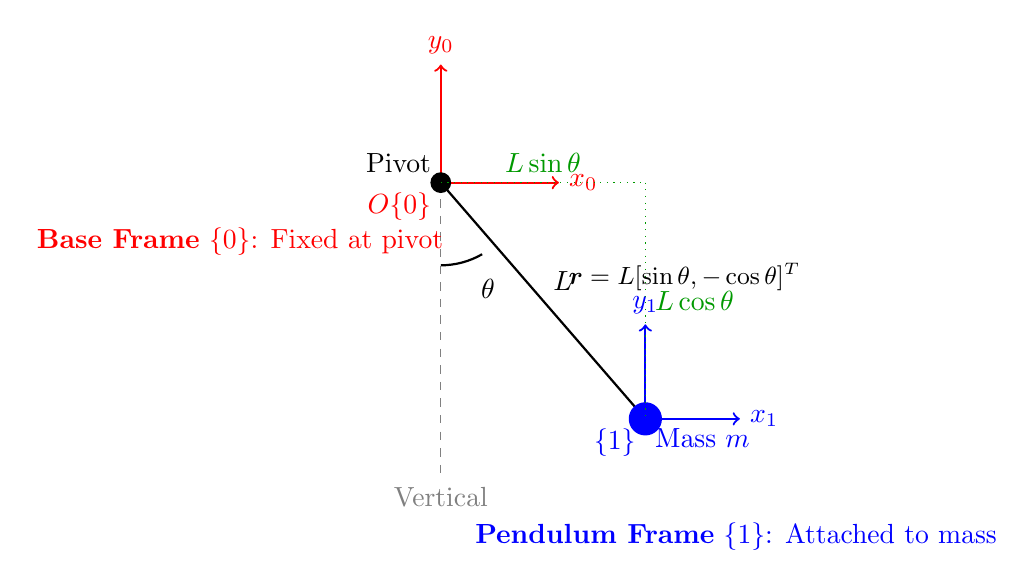
\begin{tikzpicture}[scale=1.5]
    % Grid for reference (optional, can be removed)
    %\draw[very thin,color=gray] (-0.5,-2.5) grid (3.5,1.5);
    
    % Base frame (origin)
    \draw[thick, ->, red] (0,0) -- (1,0) node[right] {$x_0$};
    \draw[thick, ->, red] (0,0) -- (0,1) node[above] {$y_0$};
    \node[below left, red] at (0,0) {$O \{0\}$};
    
    % Vertical reference line (dashed)
    \draw[dashed, gray] (0,0) -- (0,-2.5) node[below] {Vertical};
    
    % Pendulum rod
    \draw[thick, black] (0,0) -- (2*0.866, -2) node[midway, above right] {$L$};
    \fill[black] (0,0) circle (2.5pt) node[above left] {Pivot};
    \fill[blue] (2*0.866, -2) circle (4pt) node[below right] {Mass $m$};
    
    % Angle arc and label
    \draw[thick] (0,-0.7) arc (-90:-60:0.7);
    \node at (0.4,-0.9) {$\theta$};
    
    % Pendulum frame at mass location
    \draw[thick, ->, blue] (2*0.866, -2) -- (2*0.866+0.8, -2) node[right] {$x_1$};
    \draw[thick, ->, blue] (2*0.866, -2) -- (2*0.866, -2+0.8) node[above] {$y_1$};
    \node[below left, blue] at (2*0.866, -2) {$\{1\}$};
    
    % Position components
    \draw[dotted, green!60!black] (0,0) -- (2*0.866, 0) node[midway, above] {$L\sin\theta$};
    \draw[dotted, green!60!black] (2*0.866, 0) -- (2*0.866, -2) node[midway, right] {$L\cos\theta$};
    
    % Coordinate labels with better positioning
    \node[red, below] at (-1.7,-0.3) {\textbf{Base Frame} $\{0\}$: Fixed at pivot};
    \node[blue, below] at (2.5,-2.8) {\textbf{Pendulum Frame} $\{1\}$: Attached to mass};
    
    % Additional annotations
    \node[above right] at (1, -1) {\small $\bm{r} = L[\sin\theta, -\cos\theta]^T$};
\end{tikzpicture}
\caption{Simple 2D pendulum system demonstrating coordinate frame transformations. The base frame $\{0\}$ is fixed at the pivot point, while the pendulum frame $\{1\}$ moves with the mass. The position vector components and transformation angle $\theta$ are clearly illustrated.}
\label{fig:pendulum_example}
\end{figure}

\textbf{System Description:}
\begin{itemize}
    \item Base frame $\{0\}$: Fixed coordinate system at the pivot point
    \item Pendulum frame $\{1\}$: Moving coordinate system attached to the mass
    \item Length: $L$ (distance from pivot to mass)
    \item Angle: $\theta$ (measured from vertical, positive clockwise)
\end{itemize}

\textbf{Transformation Matrix Derivation:}

The transformation from base frame $\{0\}$ to pendulum frame $\{1\}$ is:
\begin{align}
\bm{T}_1^0 &= \begin{bmatrix}
\cos\theta & -\sin\theta & L\sin\theta \\
\sin\theta & \cos\theta & -L\cos\theta \\
0 & 0 & 1
\end{bmatrix}
\end{align}

\textbf{Step-by-Step Derivation:}

1) \textbf{Position of pendulum mass in base frame:}
   \begin{align}
   x_m &= L\sin\theta \\
   y_m &= -L\cos\theta
   \end{align}

2) \textbf{Orientation of pendulum frame:}
   The pendulum frame is rotated by angle $\theta$ relative to the base frame.

3) \textbf{Complete transformation:}
   \begin{align}
   \begin{bmatrix} x_1 \\ y_1 \\ 1 \end{bmatrix} &= \bm{T}_1^0 \begin{bmatrix} x_0 \\ y_0 \\ 1 \end{bmatrix} \\
   &= \begin{bmatrix}
   \cos\theta & -\sin\theta & L\sin\theta \\
   \sin\theta & \cos\theta & -L\cos\theta \\
   0 & 0 & 1
   \end{bmatrix} \begin{bmatrix} x_0 \\ y_0 \\ 1 \end{bmatrix}
   \end{align}

\textbf{Numerical Example:}

For $\theta = 30^{\circ}$ and $L = 1$ meter:
\begin{align}
\bm{T}_1^0 &= \begin{bmatrix}
\cos(30^{\circ}) & -\sin(30^{\circ}) & 1 \cdot \sin(30^{\circ}) \\
\sin(30^{\circ}) & \cos(30^{\circ}) & -1 \cdot \cos(30^{\circ}) \\
0 & 0 & 1
\end{bmatrix} \\
&= \begin{bmatrix}
0.866 & -0.5 & 0.5 \\
0.5 & 0.866 & -0.866 \\
0 & 0 & 1
\end{bmatrix}
\end{align}

\textbf{Verification:}
The origin of frame $\{1\}$ (pendulum mass position) in frame $\{0\}$:
\begin{align}
\begin{bmatrix} x_m \\ y_m \\ 1 \end{bmatrix} &= \bm{T}_1^0 \begin{bmatrix} 0 \\ 0 \\ 1 \end{bmatrix} = \begin{bmatrix} 0.5 \\ -0.866 \\ 1 \end{bmatrix}
\end{align}

This matches our geometric calculation: $x_m = L\sin(30^{\circ}) = 0.5$, $y_m = -L\cos(30^{\circ}) = -0.866$.

\textbf{Connection to Robot Analysis:}

This pendulum example demonstrates the same principles used in our robot:
\begin{enumerate}
    \item \textbf{Frame assignment:} Each moving part gets its own coordinate frame
    \item \textbf{DH-like parameterization:} Angle $\theta$ and length $L$ define the transformation
    \item \textbf{Forward kinematics:} Transformation matrix gives end-effector position
    \item \textbf{Singularity concepts:} When $\theta = 0^{\circ}$ or $180^{\circ}$, the pendulum loses a degree of freedom
\end{enumerate}

The robot's two-link structure can be viewed as two connected pendulums, making this a perfect stepping stone to understanding the more complex system.

\textbf{Specific Transformations for the Robot:}

\textit{1. Base to Joint 1 Transformation:}
Since joint 1 is located at the base origin with rotation $q_1$:
\begin{align}
\bm{T}_1^0 &= \begin{bmatrix}
\cos q_1 & -\sin q_1 & 0 \\
\sin q_1 & \cos q_1 & 0 \\
0 & 0 & 1
\end{bmatrix}
\end{align}

\textit{2. Joint 1 to Link 1 End Transformation:}
Translation along link 1 of length $l_1$:
\begin{align}
\bm{T}_{1e}^1 &= \begin{bmatrix}
1 & 0 & l_1 \\
0 & 1 & 0 \\
0 & 0 & 1
\end{bmatrix}
\end{align}

\textit{3. Link 1 End to Joint 2 Transformation:}
Rotation by angle $q_2$ at joint 2:
\begin{align}
\bm{T}_2^{1e} &= \begin{bmatrix}
\cos q_2 & -\sin q_2 & 0 \\
\sin q_2 & \cos q_2 & 0 \\
0 & 0 & 1
\end{bmatrix}
\end{align}

\textit{4. Joint 2 to End-Effector Transformation:}
Translation along link 2 of length $l_2$:
\begin{align}
\bm{T}_M^2 &= \begin{bmatrix}
1 & 0 & l_2 \\
0 & 1 & 0 \\
0 & 0 & 1
\end{bmatrix}
\end{align}

\textbf{Complete Chain Transformation:}
The transformation from base to end-effector is:
\begin{align}
\bm{T}_M^0 &= \bm{T}_1^0 \bm{T}_{1e}^1 \bm{T}_2^{1e} \bm{T}_M^2 \\
&= \begin{bmatrix}
\cos q_1 & -\sin q_1 & 0 \\
\sin q_1 & \cos q_1 & 0 \\
0 & 0 & 1
\end{bmatrix}
\begin{bmatrix}
1 & 0 & l_1 \\
0 & 1 & 0 \\
0 & 0 & 1
\end{bmatrix}
\begin{bmatrix}
\cos q_2 & -\sin q_2 & 0 \\
\sin q_2 & \cos q_2 & 0 \\
0 & 0 & 1
\end{bmatrix}
\begin{bmatrix}
1 & 0 & l_2 \\
0 & 1 & 0 \\
0 & 0 & 1
\end{bmatrix}
\end{align}

\textbf{Simplified End-Effector Transformation:}
After matrix multiplication, the final transformation becomes:
\begin{align}
\bm{T}_M^0 &= \begin{bmatrix}
\cos(q_1 + q_2) & -\sin(q_1 + q_2) & l_1\cos q_1 + l_2\cos(q_1 + q_2) \\
\sin(q_1 + q_2) & \cos(q_1 + q_2) & l_1\sin q_1 + l_2\sin(q_1 + q_2) \\
0 & 0 & 1
\end{bmatrix}
\end{align}

\textbf{Cable Anchor Transformations:}
For cable analysis, we need transformations from the base frame to cable anchor points:

\textit{Left Cable Anchor:}
\begin{align}
\bm{T}_{A1}^0 &= \begin{bmatrix}
1 & 0 & -L \\
0 & 1 & 0 \\
0 & 0 & 1
\end{bmatrix}
\end{align}

\textit{Right Cable Anchor:}
\begin{align}
\bm{T}_{A2}^0 &= \begin{bmatrix}
1 & 0 & L \\
0 & 1 & 0 \\
0 & 0 & 1
\end{bmatrix}
\end{align}

\textbf{Point Transformation:}
To transform a point $\bm{p}_i$ from frame $\{i\}$ to frame $\{j\}$:
\begin{align}
\bm{p}_j &= \bm{T}_j^i \begin{bmatrix} \bm{p}_i \\ 1 \end{bmatrix} \\
\begin{bmatrix} x_j \\ y_j \\ 1 \end{bmatrix} &= \begin{bmatrix}
\cos\theta & -\sin\theta & x_{trans} \\
\sin\theta & \cos\theta & y_{trans} \\
0 & 0 & 1
\end{bmatrix} \begin{bmatrix} x_i \\ y_i \\ 1 \end{bmatrix}
\end{align}

\textbf{Vector Transformation:}
To transform a vector $\bm{v}_i$ (direction only):
\begin{align}
\bm{v}_j &= \bm{R}_j^i \bm{v}_i \\
\begin{bmatrix} v_{x,j} \\ v_{y,j} \end{bmatrix} &= \begin{bmatrix}
\cos\theta & -\sin\theta \\
\sin\theta & \cos\theta
\end{bmatrix} \begin{bmatrix} v_{x,i} \\ v_{y,i} \end{bmatrix}
\end{align}

\textbf{Applications in Singularity Analysis:}
Transformation matrices are crucial for:
\begin{enumerate}
    \item \textbf{Jacobian Computation:} Relating joint velocities to end-effector velocities
    \item \textbf{Cable Vector Calculation:} Determining cable directions in different frames
    \item \textbf{Force Transformation:} Converting forces between coordinate frames
    \item \textbf{Workspace Analysis:} Mapping reachable positions and orientations
\end{enumerate}

\subsubsection{Denavit-Hartenberg Parameters}
The Denavit-Hartenberg (DH) convention provides a systematic method for describing the kinematic structure of serial manipulators. For the 2-DOF planar serial chain, we establish the DH parameters that define the relationship between consecutive coordinate frames.

\textbf{DH Convention Rules:}
The DH convention defines four parameters for each link:
\begin{itemize}
    \item $a_i$: Link length - distance from $z_{i-1}$ to $z_i$ along $x_i$
    \item $\alpha_i$: Link twist - angle from $z_{i-1}$ to $z_i$ about $x_i$
    \item $d_i$: Link offset - distance from $x_{i-1}$ to $x_i$ along $z_{i-1}$
    \item $\theta_i$: Joint angle - angle from $x_{i-1}$ to $x_i$ about $z_{i-1}$
\end{itemize}

\textbf{Frame Assignment for 2-DOF Planar Robot:}

\textit{Frame 0 (Base Frame):}
\begin{itemize}
    \item Origin at joint 1 center
    \item $z_0$-axis: perpendicular to the plane (pointing out of page)
    \item $x_0$-axis: along the initial direction of link 1
    \item $y_0$-axis: completes the right-hand coordinate system
\end{itemize}

\textit{Frame 1 (After Joint 1):}
\begin{itemize}
    \item Origin at joint 2 center (end of link 1)
    \item $z_1$-axis: parallel to $z_0$ (planar motion)
    \item $x_1$-axis: along the direction of link 2
    \item $y_1$-axis: completes the right-hand coordinate system
\end{itemize}

\textit{Frame 2 (End-Effector Frame):}
\begin{itemize}
    \item Origin at end-effector point M
    \item $z_2$-axis: parallel to $z_0$ and $z_1$
    \item $x_2$-axis: along the final link direction
    \item $y_2$-axis: completes the right-hand coordinate system
\end{itemize}

\textbf{DH Parameters for the 2-DOF Planar Robot:}
\begin{table}[h]
\centering
\begin{tabular}{|c|c|c|c|c|c|}
\hline
Link & $a_i$ & $\alpha_i$ & $d_i$ & $\theta_i$ & Description \\
\hline
1 & $l_1$ & $0$ & $0$ & $q_1^*$ & First revolute joint \\
2 & $l_2$ & $0$ & $0$ & $q_2^*$ & Second revolute joint \\
\hline
\end{tabular}
\caption{Denavit-Hartenberg parameters for 2-DOF planar serial chain}
\label{tab:dh_parameters}
\end{table}

Where $q_i^*$ indicates that $\theta_i = q_i$ (joint variable).

\textbf{Detailed Parameter Justification:}

\textit{Link 1 Parameters:}
\begin{align}
a_1 &= l_1 \quad \text{(length of link 1)} \\
\alpha_{DH,1} &= 0 \quad \text{(planar motion, no twist)} \\
d_1 &= 0 \quad \text{(revolute joint, no offset)} \\
\theta_1 &= q_1 \quad \text{(joint variable)}
\end{align}

\textit{Link 2 Parameters:}
\begin{align}
a_2 &= l_2 \quad \text{(length of link 2)} \\
\alpha_{DH,2} &= 0 \quad \text{(planar motion, no twist)} \\
d_2 &= 0 \quad \text{(revolute joint, no offset)} \\
\theta_2 &= q_2 \quad \text{(joint variable)}
\end{align}

\textbf{DH Transformation Matrix:}
The standard DH transformation matrix from frame $i-1$ to frame $i$ is:
\begin{align}
\bm{T}_i^{i-1} &= \text{Rot}_{z}(\theta_i) \cdot \text{Trans}_{z}(d_i) \cdot \text{Trans}_{x}(a_i) \cdot \text{Rot}_{x}(\alpha_i) \\
&= \begin{bmatrix}
\cos\theta_i & -\sin\theta_i\cos\alpha_i & \sin\theta_i\sin\alpha_i & a_i\cos\theta_i \\
\sin\theta_i & \cos\theta_i\cos\alpha_i & -\cos\theta_i\sin\alpha_i & a_i\sin\theta_i \\
0 & \sin\alpha_i & \cos\alpha_i & d_i \\
0 & 0 & 0 & 1
\end{bmatrix}
\end{align}

\textbf{Simplified 2D Planar Case:}
For planar motion ($\alpha_i = 0$, $d_i = 0$), the transformation simplifies to:
\begin{align}
\bm{T}_i^{i-1} &= \begin{bmatrix}
\cos\theta_i & -\sin\theta_i & a_i\cos\theta_i \\
\sin\theta_i & \cos\theta_i & a_i\sin\theta_i \\
0 & 0 & 1
\end{bmatrix}
\end{align}

\textbf{Individual Link Transformations:}

\textit{Base to Frame 1 (Joint 1):}
\begin{align}
\bm{T}_1^0 &= \begin{bmatrix}
\cos q_1 & -\sin q_1 & l_1\cos q_1 \\
\sin q_1 & \cos q_1 & l_1\sin q_1 \\
0 & 0 & 1
\end{bmatrix}
\end{align}

\textit{Frame 1 to Frame 2 (Joint 2):}
\begin{align}
\bm{T}_2^1 &= \begin{bmatrix}
\cos q_2 & -\sin q_2 & l_2\cos q_2 \\
\sin q_2 & \cos q_2 & l_2\sin q_2 \\
0 & 0 & 1
\end{bmatrix}
\end{align}

\textbf{Forward Kinematics via DH Parameters:}
The complete transformation from base to end-effector:
\begin{align}
\bm{T}_2^0 &= \bm{T}_1^0 \bm{T}_2^1 \\
&= \begin{bmatrix}
\cos q_1 & -\sin q_1 & l_1\cos q_1 \\
\sin q_1 & \cos q_1 & l_1\sin q_1 \\
0 & 0 & 1
\end{bmatrix}
\begin{bmatrix}
\cos q_2 & -\sin q_2 & l_2\cos q_2 \\
\sin q_2 & \cos q_2 & l_2\sin q_2 \\
0 & 0 & 1
\end{bmatrix}
\end{align}

After multiplication:
\begin{align}
\bm{T}_2^0 &= \begin{bmatrix}
\cos(q_1+q_2) & -\sin(q_1+q_2) & l_1\cos q_1 + l_2\cos(q_1+q_2) \\
\sin(q_1+q_2) & \cos(q_1+q_2) & l_1\sin q_1 + l_2\sin(q_1+q_2) \\
0 & 0 & 1
\end{bmatrix}
\end{align}

\textbf{End-Effector Position:}
From the transformation matrix, the end-effector position is:
\begin{align}
\bm{p}_M &= \begin{bmatrix} x_M \\ y_M \end{bmatrix} = \begin{bmatrix}
l_1\cos q_1 + l_2\cos(q_1+q_2) \\
l_1\sin q_1 + l_2\sin(q_1+q_2)
\end{bmatrix}
\end{align}

\textbf{Validation of DH Parameters:}
The DH parameters can be validated by checking:
\begin{enumerate}
    \item \textbf{Workspace boundary:} Maximum reach = $l_1 + l_2$, minimum reach = $|l_1 - l_2|$
    \item \textbf{Joint limits:} Typical range $q_i \in [-\pi, \pi]$ for full rotation
    \item \textbf{Singularity conditions:} When $q_2 = 0$ or $q_2 = \pi$ (extended/folded)
    \item \textbf{Frame consistency:} Right-hand rule preserved through all transformations
\end{enumerate}

\textbf{Alternative DH Conventions:}
Note that some literature uses modified DH parameters. The relationship between standard and modified DH is:
\begin{align}
\bm{T}_{i,modified}^{i-1} &= \text{Rot}_{x}(\alpha_{i-1}) \cdot \text{Trans}_{x}(a_{i-1}) \cdot \text{Rot}_{z}(\theta_i) \cdot \text{Trans}_{z}(d_i)
\end{align}

For our planar robot, both conventions yield the same result due to $\alpha_i = 0$ and $d_i = 0$.

\textbf{Applications in Singularity Analysis:}
DH parameters are fundamental for:
\begin{enumerate}
    \item \textbf{Jacobian derivation:} Systematic computation of velocity relationships
    \item \textbf{Workspace analysis:} Determining reachable positions and orientations
    \item \textbf{Inverse kinematics:} Solving for joint angles given end-effector pose
    \item \textbf{Dynamic modeling:} Computing inertia matrices and Coriolis terms
\end{enumerate}

\section{Forward Kinematics}

\subsection{Serial Chain Kinematics}
For the 2-DOF serial chain, the forward kinematics are:

\subsubsection{Joint 2 Position (Elbow)}
\begin{align}
\bm{p}_A &= \begin{bmatrix} x_A \\ y_A \end{bmatrix} = \begin{bmatrix} l_1 \cos q_1 \\ l_1 \sin q_1 \end{bmatrix}
\end{align}

\subsubsection{End-Effector Position}
\begin{align}
\bm{p}_M &= \begin{bmatrix} x_M \\ y_M \end{bmatrix} \\
&= \bm{p}_A + l_2 \begin{bmatrix} \cos(q_1 + q_2) \\ \sin(q_1 + q_2) \end{bmatrix} \\
&= \begin{bmatrix} l_1 \cos q_1 + l_2 \cos(q_1 + q_2) \\ l_1 \sin q_1 + l_2 \sin(q_1 + q_2) \end{bmatrix}
\end{align}

\subsubsection{Transformation Matrices}

\textbf{Derivation of Transformation Matrices:}

The transformation matrices are derived systematically using the Denavit-Hartenberg parameters established in the previous section. We'll show the step-by-step derivation for each transformation.

\textbf{Step 1: Base to Frame 1 Transformation ($\bm{T}_1^0$)}

Starting from the DH parameters for link 1:
- $a_1 = l_1$, $\alpha_{DH,1} = 0$, $d_1 = 0$, $\theta_1 = q_1$

The general DH transformation matrix is:
\begin{align}
\bm{T}_i^{i-1} &= \begin{bmatrix}
\cos\theta_i & -\sin\theta_i\cos\alpha_i & \sin\theta_i\sin\alpha_i & a_i\cos\theta_i \\
\sin\theta_i & \cos\theta_i\cos\alpha_i & -\cos\theta_i\sin\alpha_i & a_i\sin\theta_i \\
0 & \sin\alpha_i & \cos\alpha_i & d_i \\
0 & 0 & 0 & 1
\end{bmatrix}
\end{align}

Substituting the parameters for link 1 ($\theta_1 = q_1$, $\alpha_1 = 0$, $d_1 = 0$, $a_1 = l_1$):
\begin{align}
\cos\alpha_{DH,1} &= \cos(0) = 1 \\
\sin\alpha_{DH,1} &= \sin(0) = 0
\end{align}

Therefore:
\begin{align}
\bm{T}_1^0 &= \begin{bmatrix}
\cos q_1 & -\sin q_1 \cdot 1 & \sin q_1 \cdot 0 & l_1\cos q_1 \\
\sin q_1 & \cos q_1 \cdot 1 & -\cos q_1 \cdot 0 & l_1\sin q_1 \\
0 & 0 & 1 & 0 \\
0 & 0 & 0 & 1
\end{bmatrix} \\
&= \begin{bmatrix}
\cos q_1 & -\sin q_1 & 0 & l_1\cos q_1 \\
\sin q_1 & \cos q_1 & 0 & l_1\sin q_1 \\
0 & 0 & 1 & 0 \\
0 & 0 & 0 & 1
\end{bmatrix}
\end{align}

For 2D planar motion, we reduce this to:
\begin{align}
\bm{T}_1^0 &= \begin{bmatrix}
\cos q_1 & -\sin q_1 & l_1\cos q_1 \\
\sin q_1 & \cos q_1 & l_1\sin q_1 \\
0 & 0 & 1
\end{bmatrix}
\end{align}

\textbf{Physical Interpretation:}
This transformation represents:
\begin{itemize}
    \item \textbf{Rotation by $q_1$}: The $2 \times 2$ rotation submatrix rotates frame 0 by angle $q_1$
    \item \textbf{Translation by $l_1$}: The translation vector moves along the rotated $x_1$-axis by distance $l_1$
\end{itemize}

\textbf{Step 2: Frame 1 to Frame 2 Transformation ($\bm{T}_2^1$)}

For link 2 with DH parameters:
- $a_2 = l_2$, $\alpha_{DH,2} = 0$, $d_2 = 0$, $\theta_2 = q_2$

Following the same process:
\begin{align}
\bm{T}_2^1 &= \begin{bmatrix}
\cos q_2 & -\sin q_2 & l_2\cos q_2 \\
\sin q_2 & \cos q_2 & l_2\sin q_2 \\
0 & 0 & 1
\end{bmatrix}
\end{align}

\textbf{Step 3: Complete Chain Transformation ($\bm{T}_2^0$)}

The complete transformation from base to end-effector is obtained by matrix multiplication:
\begin{align}
\bm{T}_2^0 &= \bm{T}_1^0 \bm{T}_2^1 \\
&= \begin{bmatrix}
\cos q_1 & -\sin q_1 & l_1\cos q_1 \\
\sin q_1 & \cos q_1 & l_1\sin q_1 \\
0 & 0 & 1
\end{bmatrix}
\begin{bmatrix}
\cos q_2 & -\sin q_2 & l_2\cos q_2 \\
\sin q_2 & \cos q_2 & l_2\sin q_2 \\
0 & 0 & 1
\end{bmatrix}
\end{align}

\textbf{Detailed Matrix Multiplication:}

Let's compute each element of the result matrix $\bm{T}_2^0$:

\textit{Rotation Matrix Elements (upper-left $2 \times 2$):}
\begin{align}
R_{11} &= \cos q_1 \cos q_2 - (-\sin q_1)(\sin q_2) = \cos q_1 \cos q_2 + \sin q_1 \sin q_2 = \cos(q_1 + q_2) \\
R_{12} &= \cos q_1(-\sin q_2) - (-\sin q_1)(\cos q_2) = -\cos q_1 \sin q_2 + \sin q_1 \cos q_2 = -\sin(q_1 + q_2) \\
R_{21} &= \sin q_1 \cos q_2 - \cos q_1 \sin q_2 = \sin q_1 \cos q_2 - \cos q_1 \sin q_2 = \sin(q_1 + q_2) \\
R_{22} &= \sin q_1(-\sin q_2) - \cos q_1(-\cos q_2) = -\sin q_1 \sin q_2 + \cos q_1 \cos q_2 = \cos(q_1 + q_2)
\end{align}

\textit{Translation Vector Elements:}
\begin{align}
T_x &= \cos q_1 (l_2\cos q_2) + (-\sin q_1)(l_2\sin q_2) + l_1\cos q_1 \\
&= l_2(\cos q_1 \cos q_2 - \sin q_1 \sin q_2) + l_1\cos q_1 \\
&= l_2\cos(q_1 + q_2) + l_1\cos q_1 \\
T_y &= \sin q_1 (l_2\cos q_2) + \cos q_1 (l_2\sin q_2) + l_1\sin q_1 \\
&= l_2(\sin q_1 \cos q_2 + \cos q_1 \sin q_2) + l_1\sin q_1 \\
&= l_2\sin(q_1 + q_2) + l_1\sin q_1
\end{align}

\textbf{Final Result:}
\begin{align}
\bm{T}_2^0 &= \begin{bmatrix}
\cos(q_1 + q_2) & -\sin(q_1 + q_2) & l_1\cos q_1 + l_2\cos(q_1 + q_2) \\
\sin(q_1 + q_2) & \cos(q_1 + q_2) & l_1\sin q_1 + l_2\sin(q_1 + q_2) \\
0 & 0 & 1
\end{bmatrix}
\end{align}

\textbf{Verification Using Trigonometric Identities:}

The derivation uses the angle addition formulas:
\begin{align}
\cos(A + B) &= \cos A \cos B - \sin A \sin B \\
\sin(A + B) &= \sin A \cos B + \cos A \sin B
\end{align}

Where $A = q_1$ and $B = q_2$.

\textbf{Alternative Derivation - Geometric Approach:}

We can also derive this geometrically:
\begin{enumerate}
    \item \textbf{Joint 1 contribution:} Point moves from origin to $(l_1\cos q_1, l_1\sin q_1)$
    \item \textbf{Joint 2 contribution:} From joint 1 position, move distance $l_2$ in direction $(q_1 + q_2)$
    \item \textbf{Final position:} Sum of both contributions gives the end-effector position
\end{enumerate}

\textbf{Summary of Individual Transformations:}
\begin{align}
\bm{T}_1^0 &= \begin{bmatrix}
\cos q_1 & -\sin q_1 & l_1 \cos q_1 \\
\sin q_1 & \cos q_1 & l_1 \sin q_1 \\
0 & 0 & 1
\end{bmatrix} \quad \text{(Base to Joint 2)} \\
\bm{T}_2^1 &= \begin{bmatrix}
\cos q_2 & -\sin q_2 & l_2 \cos q_2 \\
\sin q_2 & \cos q_2 & l_2 \sin q_2 \\
0 & 0 & 1
\end{bmatrix} \quad \text{(Joint 2 to End-Effector)} \\
\bm{T}_2^0 &= \bm{T}_1^0 \bm{T}_2^1 \quad \text{(Complete Chain)}
\end{align}

\subsection{Cable Kinematics}
Both cables are attached to the end-effector point M and extend to fixed anchor points:

\subsubsection{Cable Length Equations}
Cable 1 connects anchor point $A_1 = (-L, 0)$ to end-effector M:
\begin{align}
\rho_1 &= \|\bm{p}_M - \bm{A}_1\| \\
&= \sqrt{(x_M + L)^2 + y_M^2} \\
&= \sqrt{(l_1 \cos q_1 + l_2 \cos(q_1 + q_2) + L)^2 + (l_1 \sin q_1 + l_2 \sin(q_1 + q_2))^2}
\end{align}

Cable 2 connects anchor point $A_2 = (L, 0)$ to end-effector M:
\begin{align}
\rho_2 &= \|\bm{p}_M - \bm{A}_2\| \\
&= \sqrt{(x_M - L)^2 + y_M^2} \\
&= \sqrt{(l_1 \cos q_1 + l_2 \cos(q_1 + q_2) - L)^2 + (l_1 \sin q_1 + l_2 \sin(q_1 + q_2))^2}
\end{align}

\subsubsection{Cable Direction Vectors}
The unit vectors along the cables (from anchor points toward end-effector) are:
\begin{align}
\bm{u}_1 &= \frac{\bm{p}_M - \bm{A}_1}{\rho_1} = \frac{1}{\rho_1}\begin{bmatrix} x_M + L \\ y_M \end{bmatrix} \\
\bm{u}_2 &= \frac{\bm{p}_M - \bm{A}_2}{\rho_2} = \frac{1}{\rho_2}\begin{bmatrix} x_M - L \\ y_M \end{bmatrix}
\end{align}

Alternatively, using the cable angles:
\begin{align}
\bm{u}_1 &= \begin{bmatrix} \cos\alpha_1 \\ \sin\alpha_1 \end{bmatrix} = \begin{bmatrix} \cos(\text{atan2}(y_M, x_M + L)) \\ \sin(\text{atan2}(y_M, x_M + L)) \end{bmatrix} \\
\bm{u}_2 &= \begin{bmatrix} \cos\alpha_2 \\ \sin\alpha_2 \end{bmatrix} = \begin{bmatrix} \cos(\text{atan2}(y_M, x_M - L)) \\ \sin(\text{atan2}(y_M, x_M - L)) \end{bmatrix}
\end{align}

Note that:
\begin{align}
\cos(\text{atan2}(y, x)) &= \frac{x}{\sqrt{x^2 + y^2}} \\
\sin(\text{atan2}(y, x)) &= \frac{y}{\sqrt{x^2 + y^2}}
\end{align}

\subsubsection{Cable Angles}
Using the two-argument arctangent function for proper quadrant handling:
\begin{align}
\alpha_1 &= \text{atan2}(y_M, x_M + L) \\
\alpha_2 &= \text{atan2}(y_M, x_M - L)
\end{align}

\textbf{Critical for this robot configuration:}
\begin{itemize}
    \item When $x_M = -L$: Cable 1 is vertical, $\text{atan2}(y_M, 0)$ handles this correctly
    \item When $x_M = +L$: Cable 2 is vertical, $\text{atan2}(y_M, 0)$ handles this correctly  
    \item When $y_M = 0$: Both cables horizontal, $\text{atan2}(0, x_M \pm L)$ returns $0$ or $\pi$
    \item Workspace boundaries: Continuous angle computation throughout reachable space
\end{itemize}

Where $\text{atan2}(y, x)$ returns the angle $\theta \in (-\pi, \pi]$ such that:
\begin{align}
x &= r\cos\theta \\
y &= r\sin\theta
\end{align}

This formulation:
\begin{itemize}
    \item Handles all four quadrants correctly
    \item Avoids division by zero when $x_M = -L$ or $x_M = L$
    \item Provides continuous angle values as the end-effector moves
    \item Returns angles in the range $(-\pi, \pi]$
\end{itemize}

\subsection{Complete Forward Kinematics}
In this hybrid system, the end-effector position is determined by both the serial chain configuration and cable length constraints:

\subsubsection{Primary Positioning (Serial Chain)}
The serial chain provides the primary positioning capability:
\begin{align}
\bm{p}_{M,serial} &= \begin{bmatrix} x_M \\ y_M \end{bmatrix} \\
&= \begin{bmatrix} l_1 \cos q_1 + l_2 \cos(q_1 + q_2) \\ l_1 \sin q_1 + l_2 \sin(q_1 + q_2) \end{bmatrix}
\end{align}

\subsubsection{Cable Length Constraints}
The cables impose constraints on the achievable positions:
\begin{align}
\rho_1 &= f_1(\bm{q}) = \sqrt{(x_M(\bm{q}) + L)^2 + y_M(\bm{q})^2} \\
\rho_2 &= f_2(\bm{q}) = \sqrt{(x_M(\bm{q}) - L)^2 + y_M(\bm{q})^2}
\end{align}

\subsubsection{Hybrid System Formulation}
For a given cable length pair $(\rho_1, \rho_2)$, the end-effector must satisfy:
\begin{align}
\bm{g}(\bm{q}, \bm{\rho}) &= \begin{bmatrix} g_1(\bm{q}, \rho_1) \\ g_2(\bm{q}, \rho_2) \end{bmatrix} = \bm{0}
\end{align}

Where:
\begin{align}
g_1(\bm{q}, \rho_1) &= (x_M + L)^2 + y_M^2 - \rho_1^2 = 0 \\
g_2(\bm{q}, \rho_2) &= (x_M - L)^2 + y_M^2 - \rho_2^2 = 0
\end{align}

\subsubsection{Constraint Equations}

\textbf{Important Clarification: Nature of Cable Constraints}

In a cable-driven robot, the cable lengths $\rho_1$ and $\rho_2$ are indeed \textbf{variable} - they change as the robot moves and are controlled by motors. However, the "constraints" here refer to the \textbf{geometric relationships} that must always be satisfied, not fixed length constraints.

\textbf{Types of Constraints in Hybrid Serial-Cable Systems:}

\textbf{1. Geometric Constraints (Always Satisfied):}
These are the fundamental geometric relationships that define how cable lengths relate to robot configuration:
\begin{align}
\rho_1^2 &= (x_M + L)^2 + y_M^2 \quad \text{(Left cable geometric constraint)} \\
\rho_2^2 &= (x_M - L)^2 + y_M^2 \quad \text{(Right cable geometric constraint)}
\end{align}

Where:
- $\rho_1, \rho_2$: \textbf{Variable} cable lengths (controlled inputs)
- $x_M, y_M$: End-effector position (functions of joint angles $q_1, q_2$)
- $L$: Fixed distance between cable anchor points

\textbf{2. Kinematic Constraint (Forward Kinematics):}
The end-effector position is determined by the serial joint configuration:
\begin{align}
x_M &= l_1\cos q_1 + l_2\cos(q_1 + q_2) \\
y_M &= l_1\sin q_1 + l_2\sin(q_1 + q_2)
\end{align}

\textbf{3. Cable Length Relationships:}
Substituting the kinematic equations into the geometric constraints:
\begin{align}
\rho_1^2 &= [l_1\cos q_1 + l_2\cos(q_1 + q_2) + L]^2 + [l_1\sin q_1 + l_2\sin(q_1 + q_2)]^2 \\
\rho_2^2 &= [l_1\cos q_1 + l_2\cos(q_1 + q_2) - L]^2 + [l_1\sin q_1 + l_2\sin(q_1 + q_2)]^2
\end{align}

\textbf{Different Control Scenarios:}

\textbf{Scenario A: Joint-Space Control (Serial Joints as Inputs)}
- \textbf{Inputs}: Joint angles $q_1, q_2$
- \textbf{Determined}: End-effector position $(x_M, y_M)$ via forward kinematics
- \textbf{Calculated}: Required cable lengths $\rho_1, \rho_2$ via geometric constraints
- \textbf{Constraint form}: $\rho_i = f(\bm{q})$ (cable lengths as functions of joint angles)

\textbf{Scenario B: Cable-Space Control (Cable Lengths as Inputs)}
- \textbf{Inputs}: Desired cable lengths $\rho_1, \rho_2$
- \textbf{Constraint}: The two cable length equations must be satisfied simultaneously
- \textbf{Determined}: End-effector position $(x_M, y_M)$ via constraint intersection
- \textbf{Calculated}: Required joint angles $q_1, q_2$ via inverse kinematics

\textbf{Mathematical Formulation for Cable-Space Control:}

The constraint equations become:
\begin{align}
g_1(\bm{q}, \rho_1) &= (x_M(\bm{q}) + L)^2 + y_M(\bm{q})^2 - \rho_1^2 = 0 \\
g_2(\bm{q}, \rho_2) &= (x_M(\bm{q}) - L)^2 + y_M(\bm{q})^2 - \rho_2^2 = 0
\end{align}

Where $x_M(\bm{q})$ and $y_M(\bm{q})$ are the forward kinematic functions.

\textbf{Constraint Jacobian for Cable-Space Control:}
\begin{align}
\bm{G}_q &= \frac{\partial \bm{g}}{\partial \bm{q}} = \begin{bmatrix}
\frac{\partial g_1}{\partial q_1} & \frac{\partial g_1}{\partial q_2} \\
\frac{\partial g_2}{\partial q_1} & \frac{\partial g_2}{\partial q_2}
\end{bmatrix}
\end{align}

\textbf{Physical Interpretation:}

\begin{itemize}
    \item \textbf{NOT fixed constraints}: The cables can change length freely
    \item \textbf{Geometric relationships}: Given any robot configuration, the cable lengths are geometrically determined
    \item \textbf{Control redundancy}: We can control either joints OR cable lengths, but not both independently
    \item \textbf{Constraint satisfaction}: Any feasible motion must satisfy the geometric relationships
\end{itemize}

\textbf{Example - Cable Length Calculation:}

For joint configuration $q_1 = 30^{\circ}$, $q_2 = 45^{\circ}$ with $l_1 = l_2 = 1$ m, $L = 2$ m:

\textit{Step 1: Calculate end-effector position}
\begin{align}
x_M &= 1 \cdot \cos(30^{\circ}) + 1 \cdot \cos(75^{\circ}) = 0.866 + 0.259 = 1.125 \text{ m} \\
y_M &= 1 \cdot \sin(30^{\circ}) + 1 \cdot \sin(75^{\circ}) = 0.500 + 0.966 = 1.466 \text{ m}
\end{align}

\textit{Step 2: Calculate required cable lengths}
\begin{align}
\rho_1 &= \sqrt{(1.125 + 2)^2 + (1.466)^2} = \sqrt{9.766 + 2.151} = 3.452 \text{ m} \\
\rho_2 &= \sqrt{(1.125 - 2)^2 + (1.466)^2} = \sqrt{0.766 + 2.151} = 1.708 \text{ m}
\end{align}

\textbf{Key Distinction:}
- The constraint equations don't fix the cable lengths
- They define the \textbf{required} cable lengths for any given robot configuration
- Or conversely, they define the \textbf{achievable} robot configurations for given cable lengths

\section{Jacobian Matrices}

\subsection{Velocity Kinematics}

\textbf{Notation Clarification:}
To avoid confusion, we establish clear notation for different types of lengths:
\begin{align}
l_1, l_2 &: \text{Fixed link lengths of the serial arm} \\
\rho_1, \rho_2 &: \text{Variable cable lengths (controlled inputs)} \\
\bm{\rho} &= \begin{bmatrix} \rho_1 \\ \rho_2 \end{bmatrix} \text{ (cable length vector)}
\end{align}

\textbf{Hybrid System Velocity Kinematics:}
The relationship between joint velocities, cable length rates, and end-effector velocities:
\begin{align}
\dot{\bm{x}} &= \bm{J}(\bm{q}, \bm{\rho}) \begin{bmatrix} \dot{\bm{q}} \\ \dot{\bm{\rho}} \end{bmatrix} \\
&= \begin{bmatrix} \bm{J}_q & \bm{J}_{\rho} \end{bmatrix} \begin{bmatrix} \dot{\bm{q}} \\ \dot{\bm{\rho}} \end{bmatrix}
\end{align}

Where:
\begin{itemize}
    \item $\dot{\bm{x}} = [\dot{x}_M, \dot{y}_M]^T$: End-effector velocity
    \item $\dot{\bm{q}} = [\dot{q}_1, \dot{q}_2]^T$: Joint angular velocities
    \item $\dot{\bm{\rho}} = [\dot{\rho}_1, \dot{\rho}_2]^T$: Cable length change rates
    \item $\bm{J}_q$: Serial joint Jacobian matrix
    \item $\bm{J}_{\rho}$: Cable Jacobian matrix
\end{itemize}

\textbf{Important Note on Cable Jacobian:}
In our hybrid system, both cables attach to the same end-effector point M. This means:
\begin{itemize}
    \item The cables don't directly control end-effector motion independently
    \item Cable motions are \textbf{constrained} by the serial arm configuration
    \item The effective Jacobian depends on which actuators are active (joints vs. cables)
\end{itemize}

\subsection{Serial Joint Jacobian}
The Jacobian with respect to serial joints:
\begin{align}
\bm{J}_q &= \frac{\partial \bm{f}}{\partial \bm{q}} \\
&= \begin{bmatrix}
\frac{\partial x}{\partial q_1} & \frac{\partial x}{\partial q_2} & \cdots & \frac{\partial x}{\partial q_{n_j}} \\
\frac{\partial y}{\partial q_1} & \frac{\partial y}{\partial q_2} & \cdots & \frac{\partial y}{\partial q_{n_j}} \\
\frac{\partial \theta}{\partial q_1} & \frac{\partial \theta}{\partial q_2} & \cdots & \frac{\partial \theta}{\partial q_{n_j}}
\end{bmatrix}
\end{align}

Individual elements for the 2-DOF serial chain:
\begin{align}
\frac{\partial x_M}{\partial q_1} &= -l_1 \sin q_1 - l_2 \sin(q_1 + q_2) \\
\frac{\partial x_M}{\partial q_2} &= -l_2 \sin(q_1 + q_2) \\
\frac{\partial y_M}{\partial q_1} &= l_1 \cos q_1 + l_2 \cos(q_1 + q_2) \\
\frac{\partial y_M}{\partial q_2} &= l_2 \cos(q_1 + q_2)
\end{align}

Therefore, the serial joint Jacobian is:
\begin{align}
\bm{J}_q &= \begin{bmatrix}
-l_1 \sin q_1 - l_2 \sin(q_1 + q_2) & -l_2 \sin(q_1 + q_2) \\
l_1 \cos q_1 + l_2 \cos(q_1 + q_2) & l_2 \cos(q_1 + q_2)
\end{bmatrix}
\end{align}

\subsection{Cable-Constraint Jacobian}
Since both cables attach to the same point M, we analyze the constraint Jacobian rather than a direct cable Jacobian. 

\subsubsection{Constraint Jacobian with respect to Joint Variables}
\begin{align}
\bm{G}_q &= \frac{\partial \bm{g}}{\partial \bm{q}} = \begin{bmatrix}
\frac{\partial g_1}{\partial q_1} & \frac{\partial g_1}{\partial q_2} \\
\frac{\partial g_2}{\partial q_1} & \frac{\partial g_2}{\partial q_2}
\end{bmatrix}
\end{align}

Computing the partial derivatives:
\begin{align}
\frac{\partial g_1}{\partial q_1} &= 2(x_M + L)\frac{\partial x_M}{\partial q_1} + 2y_M\frac{\partial y_M}{\partial q_1} \\
&= 2(x_M + L)(-l_1 \sin q_1 - l_2 \sin(q_1 + q_2)) + 2y_M(l_1 \cos q_1 + l_2 \cos(q_1 + q_2)) \\
\frac{\partial g_1}{\partial q_2} &= 2(x_M + L)(-l_2 \sin(q_1 + q_2)) + 2y_M(l_2 \cos(q_1 + q_2)) \\
\frac{\partial g_2}{\partial q_1} &= 2(x_M - L)(-l_1 \sin q_1 - l_2 \sin(q_1 + q_2)) + 2y_M(l_1 \cos q_1 + l_2 \cos(q_1 + q_2)) \\
\frac{\partial g_2}{\partial q_2} &= 2(x_M - L)(-l_2 \sin(q_1 + q_2)) + 2y_M(l_2 \cos(q_1 + q_2))
\end{align}

\subsubsection{Constraint Jacobian with respect to Cable Lengths}
\begin{align}
\bm{G}_\rho &= \frac{\partial \bm{g}}{\partial \bm{\rho}} = \begin{bmatrix}
-2\rho_1 & 0 \\
0 & -2\rho_2
\end{bmatrix}
\end{align}

For this robot, the end-effector position is determined by the serial chain configuration, not directly by cable lengths. However, if we consider the cables as additional constraints, we need to analyze the constraint Jacobian.

The constraint equations are:
\begin{align}
g_1(\bm{q}, \rho_1) &= \rho_1^2 - [(x_M + L)^2 + y_M^2] = 0 \\
g_2(\bm{q}, \rho_2) &= \rho_2^2 - [(x_M - L)^2 + y_M^2] = 0
\end{align}

The constraint Jacobian with respect to joint variables:
\begin{align}
\bm{G}_q &= \begin{bmatrix}
\frac{\partial g_1}{\partial q_1} & \frac{\partial g_1}{\partial q_2} \\
\frac{\partial g_2}{\partial q_1} & \frac{\partial g_2}{\partial q_2}
\end{bmatrix} \\
&= -2\begin{bmatrix}
(x_M + L)\frac{\partial x_M}{\partial q_1} + y_M\frac{\partial y_M}{\partial q_1} & (x_M + L)\frac{\partial x_M}{\partial q_2} + y_M\frac{\partial y_M}{\partial q_2} \\
(x_M - L)\frac{\partial x_M}{\partial q_1} + y_M\frac{\partial y_M}{\partial q_1} & (x_M - L)\frac{\partial x_M}{\partial q_2} + y_M\frac{\partial y_M}{\partial q_2}
\end{bmatrix}
\end{align}

The constraint Jacobian with respect to cable lengths:
\begin{align}
\bm{G}_\rho &= \begin{bmatrix}
2\rho_1 & 0 \\
0 & 2\rho_2
\end{bmatrix}
\end{align}

\section{Constraint Analysis}

\subsection{Constraint Jacobian}
The constraint Jacobian relates constraint variations to joint and cable variations:
\begin{align}
\frac{d\bm{g}}{dt} &= \frac{\partial \bm{g}}{\partial \bm{q}} \dot{\bm{q}} + \frac{\partial \bm{g}}{\partial \bm{l}} \dot{\bm{l}} = \bm{0} \\
\bm{G}_q \dot{\bm{q}} + \bm{G}_l \dot{\bm{l}} &= \bm{0}
\end{align}

Where:
\begin{align}
\bm{G}_q &= \frac{\partial \bm{g}}{\partial \bm{q}} = \begin{bmatrix}
\frac{\partial g_1}{\partial q_1} & \cdots & \frac{\partial g_1}{\partial q_{n_j}} \\
\vdots & \ddots & \vdots \\
\frac{\partial g_{n_c}}{\partial q_1} & \cdots & \frac{\partial g_{n_c}}{\partial q_{n_j}}
\end{bmatrix} \\
\bm{G}_{\rho} &= \frac{\partial \bm{g}}{\partial \bm{\rho}} = \begin{bmatrix}
\frac{\partial g_1}{\partial \rho_1} & \cdots & \frac{\partial g_1}{\partial \rho_{n_c}} \\
\vdots & \ddots & \vdots \\
\frac{\partial g_{n_c}}{\partial \rho_1} & \cdots & \frac{\partial g_{n_c}}{\partial \rho_{n_c}}
\end{bmatrix}
\end{align}

\textbf{NOTATION CORRECTION:} Fixed inconsistency - using $\bm{\rho} = [\rho_1, \rho_2]^T$ for cable lengths consistently throughout.

\subsection{Reduced Jacobian}
Assuming $\bm{G}_{\rho}$ is invertible, we can solve for cable length velocities:
\begin{align}
\dot{\bm{\rho}} &= -\bm{G}_{\rho}^{-1} \bm{G}_q \dot{\bm{q}} \\
\dot{\bm{x}} &= \bm{J}_q \dot{\bm{q}} + \bm{J}_{\rho} \dot{\bm{\rho}} \\
&= \bm{J}_q \dot{\bm{q}} + \bm{J}_{\rho} (-\bm{G}_{\rho}^{-1} \bm{G}_q \dot{\bm{q}}) \\
&= (\bm{J}_q - \bm{J}_{\rho} \bm{G}_{\rho}^{-1} \bm{G}_q) \dot{\bm{q}} \\
&= \bm{J}_{red} \dot{\bm{q}}
\end{align}

The reduced Jacobian is:
\begin{align}
\bm{J}_{red} &= \bm{J}_q - \bm{J}_{\rho} \bm{G}_{\rho}^{-1} \bm{G}_q
\end{align}

\section{Singularity Analysis}

\subsection{Classification of Singularities}
Singularities in hybrid serial-cable robots can be classified into several categories based on their physical interpretation and mathematical characteristics.

\subsection{Singularity Types}

\subsubsection{Type I: Serial Chain Singularities}
For the 2-DOF serial chain, singularities occur when:
\begin{align}
\det(\bm{J}_q) &= 0 \\
\text{where } \det(\bm{J}_q) &= l_2(-l_1 \sin q_1 \cos(q_1 + q_2) + l_1 \cos q_1 \sin(q_1 + q_2)) \\
&= l_1 l_2 \sin((q_1 + q_2) - q_1) \\
&= l_1 l_2 \sin q_2
\end{align}

Therefore, serial chain singularities occur when:
\begin{align}
\sin q_2 &= 0 \\
\Rightarrow q_2 &= 0 \text{ or } q_2 = \pi
\end{align}

These correspond to:
\begin{itemize}
    \item $q_2 = 0$: Fully extended configuration
    \item $q_2 = \pi$: Fully folded configuration  
\end{itemize}

\subsubsection{Type II: Cable Constraint Singularities}
Since both cables attach to the same point M, cable singularities occur when the constraint Jacobian $\bm{G}_q$ becomes singular, meaning the constraint equations become dependent.

\textbf{Geometric Interpretation:}
Cable singularities occur when the end-effector position cannot be uniquely determined by the cable length constraints, which happens when:

1. \textbf{Collinear Configuration:} End-effector lies on the X-axis ($y_M = 0$):
\begin{align}
\text{When } y_M = 0: \quad g_1 &= (x_M + L)^2 - \rho_1^2 = 0 \\
g_2 &= (x_M - L)^2 - \rho_2^2 = 0
\end{align}

The constraint gradients become:
\begin{align}
\nabla g_1 &= [2(x_M + L), 0] \\
\nabla g_2 &= [2(x_M - L), 0]
\end{align}

These are parallel (linearly dependent) when $x_M = 0$.

2. \textbf{Symmetric Configuration:} End-effector on Y-axis ($x_M = 0$):
\begin{align}
\rho_1 = \rho_2 = \sqrt{L^2 + y_M^2}
\end{align}

In this case, both constraints provide the same information about the distance from the X-axis.

\textbf{Mathematical Condition:}
\begin{align}
\det(\bm{G}_q) &= 0 \\
\text{or equivalently: } \quad \text{rank}(\bm{G}_q) &< 2
\end{align}

\subsubsection{Type III: Combined Singularities}
Occur when the complete system Jacobian loses rank:
\begin{align}
\text{rank}(\bm{J}) &< 3 \\
\det(\bm{J}\bm{J}^T) &= 0 \quad \text{(for non-square Jacobians)}
\end{align}

\subsubsection{Type IV: Constraint Singularities}
Occur when the constraint Jacobian $\bm{G}_l$ becomes singular:
\begin{align}
\det(\bm{G}_l) &= 0 \\
\text{rank}(\bm{G}_l) &< n_c
\end{align}

This represents configurations where cable length constraints become dependent.

\subsubsection{Type V: Actuation Singularities}
Occur when the system cannot generate forces in certain directions:
\begin{align}
\text{rank}(\bm{J}^T) &< 3
\end{align}

\subsection{Mathematical Characterization}

\subsubsection{Screw Theory Approach}
Using screw theory, each joint and cable contributes a twist:
\begin{align}
\bm{\xi}_i &= \begin{bmatrix} \bm{\omega}_i \\ \bm{v}_i \end{bmatrix} \quad \text{(joint twist)} \\
\bm{\zeta}_j &= \begin{bmatrix} \bm{0} \\ \bm{u}_j \end{bmatrix} \quad \text{(cable twist)}
\end{align}

Where $\bm{u}_j$ is the unit vector along cable $j$.

\subsubsection{Grassmann-Plücker Coordinates}
For planar motion, singularities can be analyzed using Plücker coordinates:
\begin{align}
\bm{L}_{ij} &= \bm{\xi}_i \times \bm{\xi}_j \\
\text{Singularity: } &\quad \bm{L}_{12} \cdot \bm{L}_{34} = 0
\end{align}

% Cable Tension Constraints and Negative Tension Analysis
% This comprehensive analysis is included from a separate file for better organization
\section{Cable Tension Constraints and Negative Tension Analysis}

\textbf{Fundamental Physical Constraint:}
A critical aspect of cable-driven systems is that cables can only pull, never push. This imposes strict inequality constraints on cable tensions:
\begin{align}
T_1 &\geq 0 \\
T_2 &\geq 0
\end{align}

\begin{figure}[htbp]
\centering
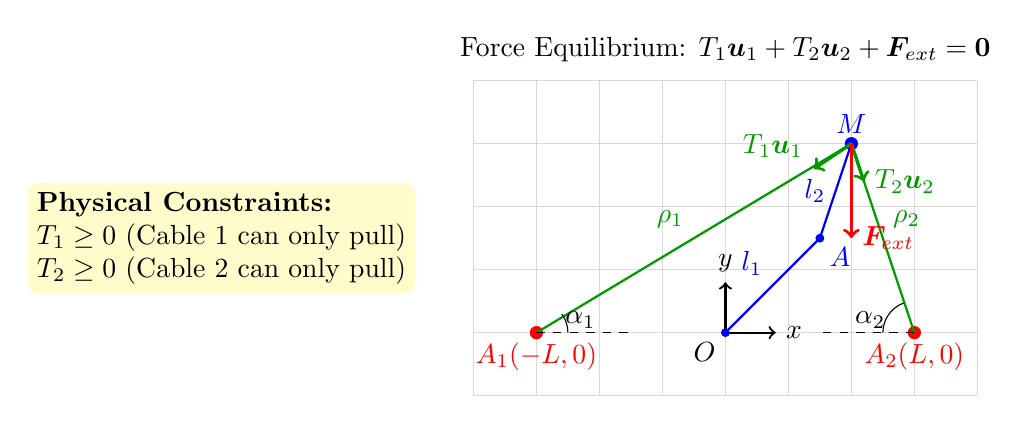
\begin{tikzpicture}[scale=0.8]
    % Grid for reference
    \draw[very thin,color=gray!30] (-4,-1) grid (4,4);
    
    % Cable anchor points
    \fill[red] (-3,0) circle (3pt) node[below] {$A_1(-L,0)$};
    \fill[red] (3,0) circle (3pt) node[below] {$A_2(L,0)$};
    
    % Base frame and robot arm (example configuration)
    \draw[thick, ->] (0,0) -- (0.8,0) node[right] {$x$};
    \draw[thick, ->] (0,0) -- (0,0.8) node[above] {$y$};
    \node[below left] at (0,0) {$O$};
    
    % Robot links (example position)
    \draw[thick, blue] (0,0) -- (1.5,1.5) node[midway, above left] {$l_1$};
    \draw[thick, blue] (1.5,1.5) -- (2,3) node[midway,  left] {$l_2$};
    
    % Joint points
    \fill[blue] (0,0) circle (2pt);
    \fill[blue] (1.5,1.5) circle (2pt) node[below right] {$A$};
    \fill[blue] (2,3) circle (3pt) node[above] {$M$};
    
    % Cables
    \draw[thick, green!60!black] (-3,0) -- (2,3) node[midway, above left] {$\rho_1$};
    \draw[thick, green!60!black] (3,0) -- (2,3) node[midway, above right] {$\rho_2$};
    
    % Cable angles
    \draw[dashed] (-3,0) -- (-1.5,0);
    \draw[dashed] (3,0) -- (1.5,0);
    \draw (-2.5,0) arc (0:36:0.5);
    \draw (2.5,0) arc (180:110:0.5);
    \node at (-2.3,0.2) {$\alpha_1$};
    \node at (2.3,0.2) {$\alpha_2$};
    
    % Cable tensions (arrows)
    \draw[->, very thick, green!60!black] (2,3) -- (1.4,2.6) node[above left] {$T_1\bm{u}_1$};
    \draw[->, very thick, green!60!black] (2,3) -- (2.2,2.4) node[right] {$T_2\bm{u}_2$};
    
    % External force
    \draw[->, very thick, red] (2,3) -- (2,1.5) node[right] {$\bm{F}_{ext}$};
    
    % Equilibrium equation
    \node[align=center] at (0,4.5) {Force Equilibrium: $T_1\bm{u}_1 + T_2\bm{u}_2 + \bm{F}_{ext} = \bm{0}$};
    
    % Constraint annotations
    \node[align=left, fill=yellow!20, rounded corners] at (-8,1.5) {
        \textbf{Physical Constraints:} \\
        $T_1 \geq 0$ (Cable 1 can only pull) \\
        $T_2 \geq 0$ (Cable 2 can only pull)
    };
\end{tikzpicture}
\caption{Cable tension force equilibrium at end-effector point M. The system must satisfy both force equilibrium and non-negative tension constraints simultaneously.}
\label{fig:cable_tension_equilibrium}
\end{figure}

\subsection{Negative Cable Tension Problem}
When mathematical analysis yields negative cable tensions, the system cannot achieve the desired force equilibrium through cables alone. This represents a fundamental limitation of cable actuation.

\textbf{Force Equilibrium Equations:}
For static equilibrium at the end-effector point M under external load $\bm{F}_{ext}$:
\begin{align}
\bm{F}_1 + \bm{F}_2 + \bm{F}_{ext} &= \bm{0} \\
T_1 \bm{u}_1 + T_2 \bm{u}_2 + \bm{F}_{ext} &= \bm{0}
\end{align}

Expanding in component form:
\begin{align}
T_1 \frac{x_M + L}{\rho_1} + T_2 \frac{x_M - L}{\rho_2} &= -F_{ext,x} \\
T_1 \frac{y_M}{\rho_1} + T_2 \frac{y_M}{\rho_2} &= -F_{ext,y}
\end{align}

\subsection{Solving for Cable Tensions}

The goal is to determine the cable tensions $T_1$ and $T_2$ required to maintain equilibrium at the end-effector point $M$ under an external force $\bm{F}_{ext} = [F_{ext,x}, F_{ext,y}]^T$. This is solved using static equilibrium conditions.

\subsubsection{Force Equilibrium at End-Effector}

At point $M$, the sum of all forces must equal zero:
\begin{align}
T_1 \bm{u}_1 + T_2 \bm{u}_2 + \bm{F}_{ext} = \bm{0}
\end{align}

Where $\bm{u}_1$ and $\bm{u}_2$ are unit vectors along the cable directions:
\begin{align}
\bm{u}_1 &= \frac{1}{\rho_1} \begin{bmatrix} x_M + L \\ y_M \end{bmatrix} \\
\bm{u}_2 &= \frac{1}{\rho_2} \begin{bmatrix} x_M - L \\ y_M \end{bmatrix}
\end{align}

\subsubsection{Matrix Formulation (Recommended for Implementation)}

The force equilibrium can be expressed as a 2×2 linear system:
\begin{align}
\begin{bmatrix}
\frac{x_M + L}{\rho_1} & \frac{x_M - L}{\rho_2} \\
\frac{y_M}{\rho_1} & \frac{y_M}{\rho_2}
\end{bmatrix} \begin{bmatrix} T_1 \\ T_2 \end{bmatrix} = -\begin{bmatrix} F_{ext,x} \\ F_{ext,y} \end{bmatrix}
\end{align}

This can be written compactly as:
\begin{align}
\bm{G}_{\rho}(\bm{q}, \bm{\rho}) \begin{bmatrix} T_1 \\ T_2 \end{bmatrix} = -\bm{F}_{ext}
\end{align}

Where $\bm{G}_{\rho}$ is the **Cable Geometry Jacobian** (also called the Constraint Jacobian), which maps cable tensions to end-effector forces.

\subsubsection{Direct Solution via Matrix Inversion}

Solving for tensions by inverting the Cable Geometry Jacobian:
\begin{align}
\begin{bmatrix} T_1 \\ T_2 \end{bmatrix} &= -\bm{G}_{\rho}^{-1}(\bm{q}, \bm{\rho}) \begin{bmatrix} F_{ext,x} \\ F_{ext,y} \end{bmatrix}
\end{align}

The determinant and inverse of the Cable Geometry Jacobian:
\begin{align}
\det(\bm{G}_{\rho}) &= \frac{1}{\rho_1 \rho_2} \left[ \frac{x_M + L}{\rho_1} \cdot \frac{y_M}{\rho_2} - \frac{x_M - L}{\rho_2} \cdot \frac{y_M}{\rho_1} \right] \\
&= \frac{y_M}{\rho_1^2 \rho_2^2} \left[ (x_M + L) - (x_M - L) \right] \\
&= \frac{2L y_M}{\rho_1^2 \rho_2^2}
\end{align}

The matrix inverse:
\begin{align}
\bm{G}_{\rho}^{-1} &= \frac{\rho_1 \rho_2}{2L y_M} \begin{bmatrix}
\frac{y_M}{\rho_2} & -\frac{x_M - L}{\rho_2} \\
-\frac{y_M}{\rho_1} & \frac{x_M + L}{\rho_1}
\end{bmatrix}
\end{align}

\subsubsection{Explicit Cable Tension Formulas}

Multiplying out the matrix inversion:
\begin{align}
T_1 &= -\frac{\rho_1}{2L} \left[ F_{ext,x} \frac{y_M}{\rho_2} - F_{ext,y} \frac{x_M - L}{\rho_2} \right] \\
&= \frac{\rho_1}{2L y_M} \left[ F_{ext,x} y_M - F_{ext,y} (x_M - L) \right] \\
T_2 &= -\frac{\rho_2}{2L} \left[ -F_{ext,x} \frac{y_M}{\rho_1} + F_{ext,y} \frac{x_M + L}{\rho_1} \right] \\
&= \frac{\rho_2}{2L y_M} \left[ F_{ext,x} y_M + F_{ext,y} (x_M + L) \right]
\end{align}

\subsubsection{Numerical Example}

\textbf{Given Configuration:}
\begin{itemize}
    \item Link lengths: $l_1 = 1$ m, $l_2 = 1$ m
    \item Cable anchor separation: $2L = 4$ m (so $L = 2$ m)
    \item Joint configuration: $q_1 = 30^{\circ}$, $q_2 = 45^{\circ}$
    \item External load: $\bm{F}_{ext} = [10, -5]^T$ N (rightward and downward)
\end{itemize}

\textbf{Step 1: Calculate end-effector position}
\begin{align}
x_M &= l_1 \cos(30^{\circ}) + l_2 \cos(75^{\circ}) = 0.866 + 0.259 = 1.125 \text{ m} \\
y_M &= l_1 \sin(30^{\circ}) + l_2 \sin(75^{\circ}) = 0.500 + 0.966 = 1.466 \text{ m}
\end{align}

\textbf{Step 2: Calculate cable lengths}
\begin{align}
\rho_1 &= \sqrt{(x_M + L)^2 + y_M^2} = \sqrt{(1.125 + 2)^2 + 1.466^2} = \sqrt{11.383} = 3.374 \text{ m} \\
\rho_2 &= \sqrt{(x_M - L)^2 + y_M^2} = \sqrt{(1.125 - 2)^2 + 1.466^2} = \sqrt{2.591} = 1.610 \text{ m}
\end{align}

\textbf{Step 3: Apply tension formulas}
\begin{align}
T_1 &= \frac{3.374}{2 \cdot 2 \cdot 1.466} \left[ 10 \cdot 1.466 - (-5) \cdot (1.125 - 2) \right] \\
&= \frac{3.374}{5.864} \left[ 14.66 + 4.4375 \right] \\
&= 0.575 \times 19.0975 = 10.98 \text{ N} \\
T_2 &= \frac{1.610}{2 \cdot 2 \cdot 1.466} \left[ 10 \cdot 1.466 + (-5) \cdot (1.125 + 2) \right] \\
&= \frac{1.610}{5.864} \left[ 14.66 - 15.625 \right] \\
&= 0.275 \times (-0.965) = -0.265 \text{ N}
\end{align}

\textbf{Result:} $T_1 = 10.98$ N (feasible), $T_2 = -0.265$ N (**negative - infeasible!**)

This configuration would require cable 2 to push, which is physically impossible. The end-effector cannot maintain equilibrium under this force with these joint angles.

\subsubsection{Stability and Computational Considerations}

\textbf{Singularity Issues:}
The Cable Geometry Jacobian becomes singular when:
\begin{align}
\det(\bm{G}_{\rho}) = \frac{2L y_M}{\rho_1^2 \rho_2^2} = 0
\end{align}

This occurs when $y_M = 0$, meaning the end-effector is on the horizontal line through the cable anchors. At this configuration, the cables cannot support vertical forces.

\textbf{Condition Number:}
To assess numerical stability, compute the condition number:
\begin{align}
\kappa(\bm{G}_{\rho}) = \|\bm{G}_{\rho}\| \cdot \|\bm{G}_{\rho}^{-1}\|
\end{align}

A high condition number indicates ill-conditioning and sensitivity to numerical errors. Avoid configurations where $\kappa > 100$.

\textbf{Computational Algorithm:}

\begin{algorithm}[H]
\caption{Cable Tension Computation and Feasibility Analysis}
\label{alg:cable_tension}
\begin{algorithmic}[1]
\REQUIRE Joint configuration $\bm{q} = [q_1, q_2]^T$, external force $\bm{F}_{ext} = [F_{ext,x}, F_{ext,y}]^T$
\REQUIRE Link lengths $l_1, l_2$, cable anchor separation $2L$, singularity tolerance $\epsilon_{sing}$
\ENSURE Cable tensions $T_1, T_2$ and feasibility status

\STATE \textbf{Step 1: Forward Kinematics}
\STATE $x_M \leftarrow l_1 \cos(q_1) + l_2 \cos(q_1 + q_2)$
\STATE $y_M \leftarrow l_1 \sin(q_1) + l_2 \sin(q_1 + q_2)$

\STATE \textbf{Step 2: Cable Length Computation}
\STATE $\rho_1 \leftarrow \sqrt{(x_M + L)^2 + y_M^2}$
\STATE $\rho_2 \leftarrow \sqrt{(x_M - L)^2 + y_M^2}$

\STATE \textbf{Step 3: Cable Geometry Jacobian Construction}
\STATE $\bm{G}_{\rho} \leftarrow \begin{bmatrix}
\frac{x_M + L}{\rho_1} & \frac{x_M - L}{\rho_2} \\
\frac{y_M}{\rho_1} & \frac{y_M}{\rho_2}
\end{bmatrix}$

\STATE \textbf{Step 4: Singularity Check}
\STATE $\det_{\rho} \leftarrow \text{determinant}(\bm{G}_{\rho}) = \frac{2L y_M}{\rho_1^2 \rho_2^2}$

\IF{$|\det_{\rho}| < \epsilon_{sing}$}
    \STATE \textbf{return} \{status: SINGULAR, $T_1$: undefined, $T_2$: undefined\}
    \STATE \textbf{// Configuration is singular - cannot solve for tensions}
\ENDIF

\STATE \textbf{Step 5: Solve Linear System via LU Decomposition}
\STATE $[\bm{L}, \bm{U}] \leftarrow \text{LU}(\bm{G}_{\rho})$
\STATE $\bm{y} \leftarrow \text{ForwardSubstitution}(\bm{L}, -\bm{F}_{ext})$
\STATE $\begin{bmatrix} T_1 \\ T_2 \end{bmatrix} \leftarrow \text{BackSubstitution}(\bm{U}, \bm{y})$

\STATE \textbf{Step 6: Feasibility Assessment}
\IF{$T_1 \geq 0$ \textbf{and} $T_2 \geq 0$}
    \STATE $\text{feasible} \leftarrow \text{TRUE}$
\ELSE
    \STATE $\text{feasible} \leftarrow \text{FALSE}$
    \STATE \textbf{// Record which tensions are negative}
    \IF{$T_1 < 0$} \STATE $\text{reason} \leftarrow \text{``Cable 1 would require push''}$ \ENDIF
    \IF{$T_2 < 0$} \STATE $\text{reason} \leftarrow \text{``Cable 2 would require push''}$ \ENDIF
\ENDIF

\STATE \textbf{Step 7: Condition Number Assessment (Optional)}
\STATE $\kappa \leftarrow \text{conditionNumber}(\bm{G}_{\rho})$
\IF{$\kappa > 100$}
    \STATE $\text{stability} \leftarrow \text{``ILL-CONDITIONED''}$
\ELSE
    \STATE $\text{stability} \leftarrow \text{``WELL-CONDITIONED''}$
\ENDIF

\STATE \textbf{return} $\{T_1, T_2, \text{feasible}, \text{stability}, \kappa\}$
\end{algorithmic}
\end{algorithm}

\subsubsection{Algorithm Details and Implementation Notes}

\textbf{Forward Kinematics Computation:}
The end-effector position is computed from joint angles using standard 2-DOF planar arm kinematics:
\begin{align}
x_M &= l_1 \cos(q_1) + l_2 \cos(q_1 + q_2) \\
y_M &= l_1 \sin(q_1) + l_2 \sin(q_1 + q_2)
\end{align}

\textbf{Cable Length Calculation:}
Euclidean distance from cable anchor points to end-effector:
\begin{align}
\rho_1 &= \|(x_M, y_M) - (-L, 0)\| = \sqrt{(x_M + L)^2 + y_M^2} \\
\rho_2 &= \|(x_M, y_M) - (L, 0)\| = \sqrt{(x_M - L)^2 + y_M^2}
\end{align}

\textbf{Singularity Detection:}
When $|\det(\bm{G}_{\rho})| < \epsilon_{sing}$ (typically $\epsilon_{sing} = 10^{-6}$):
\begin{align}
\frac{2L y_M}{\rho_1^2 \rho_2^2} \approx 0 \quad \Rightarrow \quad y_M \approx 0
\end{align}
This indicates the end-effector is near the line connecting cable anchors, where cable geometry cannot support arbitrary forces.

\textbf{Numerical Solution:}
LU decomposition is preferred over direct matrix inversion for numerical stability:
\begin{itemize}
    \item \textbf{Computational Cost}: $\mathcal{O}(n^3)$ for LU factorization (here $n=2$ is small)
    \item \textbf{Numerical Stability}: Better conditioning than explicit inversion
    \item \textbf{Reusability}: If multiple forces are applied with same configuration, LU factors can be reused
\end{itemize}

\textbf{Feasibility Criteria:}
\begin{align}
\text{Configuration is feasible} \iff T_1 \geq 0 \text{ and } T_2 \geq 0
\end{align}

\textbf{Condition Number Interpretation:}
\begin{align}
\kappa(\bm{G}_{\rho}) = \begin{cases}
< 10 & \text{Excellent conditioning} \\
10 - 100 & \text{Good conditioning} \\
100 - 1000 & \text{Moderate conditioning - use caution} \\
> 1000 & \text{Poor conditioning - near singularity}
\end{cases}
\end{align}

\subsubsection{Python Implementation Pseudocode}

\begin{verbatim}
def compute_cable_tensions(q1, q2, F_ext_x, F_ext_y, l1, l2, L, eps_sing=1e-6):
    """
    Compute cable tensions and feasibility for given configuration and external force.
    
    Parameters:
        q1, q2: Joint angles [rad]
        F_ext_x, F_ext_y: External force components [N]
        l1, l2: Link lengths [m]
        L: Half-distance between cable anchors [m]
        eps_sing: Singularity tolerance
    
    Returns:
        T1, T2: Cable tensions [N]
        feasible: Boolean indicating if tensions are non-negative
        det_G: Determinant of Cable Geometry Jacobian
        kappa: Condition number
    """
    # Step 1: Forward kinematics
    x_M = l1 * cos(q1) + l2 * cos(q1 + q2)
    y_M = l1 * sin(q1) + l2 * sin(q1 + q2)
    
    # Step 2: Cable lengths
    rho1 = sqrt((x_M + L)**2 + y_M**2)
    rho2 = sqrt((x_M - L)**2 + y_M**2)
    
    # Step 3: Cable Geometry Jacobian
    G_rho = np.array([
        [(x_M + L)/rho1, (x_M - L)/rho2],
        [y_M/rho1, y_M/rho2]
    ])
    
    # Step 4: Singularity check
    det_G = (2 * L * y_M) / (rho1**2 * rho2**2)
    if abs(det_G) < eps_sing:
        return None, None, "SINGULAR", det_G, None
    
    # Step 5: Solve for tensions
    F_ext = np.array([[-F_ext_x], [-F_ext_y]])
    T = np.linalg.solve(G_rho, F_ext)
    T1, T2 = T[0, 0], T[1, 0]
    
    # Step 6: Check feasibility
    feasible = (T1 >= 0) and (T2 >= 0)
    
    # Step 7: Condition number
    kappa = np.linalg.cond(G_rho)
    
    return T1, T2, feasible, det_G, kappa
\end{verbatim}

\subsection{Conditions for Negative Tensions}
Cable tensions become negative when:
\begin{align}
T_1 &< 0 \quad \text{or} \quad T_2 < 0
\end{align}

This occurs when the required force direction cannot be achieved by the available cable geometry.

\begin{figure}[htbp]
\centering
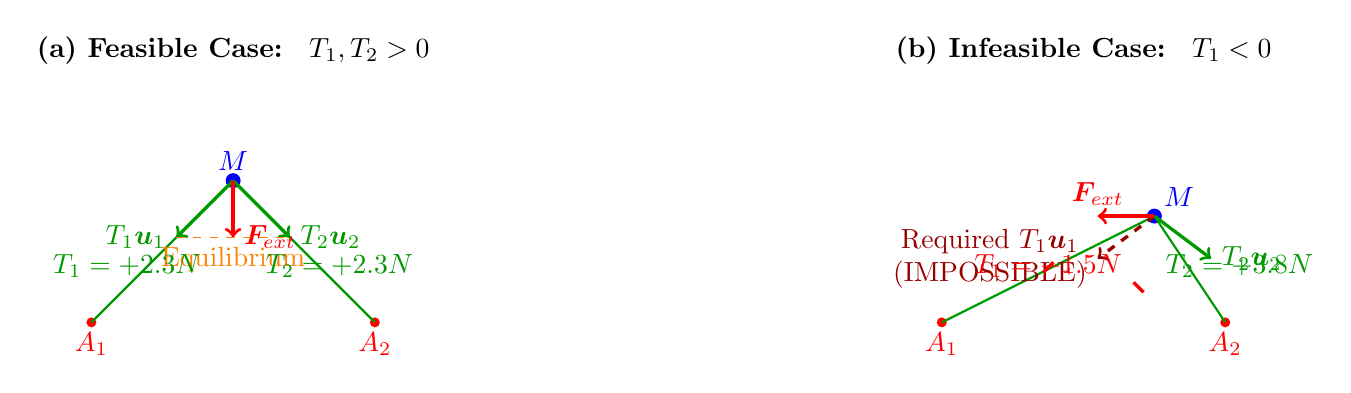
\begin{tikzpicture}[scale=0.9]
    \begin{scope}[xshift=-6cm]
        % Scenario 1: Feasible case
        \node[above] at (0,3.5) {\textbf{(a) Feasible Case: } $T_1, T_2 > 0$};
        
        % Cable anchors
        \fill[red] (-2,0) circle (2pt) node[below] {$A_1$};
        \fill[red] (2,0) circle (2pt) node[below] {$A_2$};
        
        % End-effector
        \fill[blue] (0,2) circle (3pt) node[above] {$M$};
        
        % Cables
        \draw[thick, green!60!black] (-2,0) -- (0,2);
        \draw[thick, green!60!black] (2,0) -- (0,2);
        
        % Cable forces (both pulling toward anchors)
        \draw[->, very thick, green!60!black] (0,2) -- (-0.8,1.2) node[left] {$T_1\bm{u}_1$};
        \draw[->, very thick, green!60!black] (0,2) -- (0.8,1.2) node[right] {$T_2\bm{u}_2$};
        
        % External force (downward)
        \draw[->, very thick, red] (0,2) -- (0,1.2) node[right] {$\bm{F}_{ext}$};
        
        % Force resultant (equilibrium)
        \draw[dashed, orange] (-0.8,1.2) -- (0,1.2) -- (0.8,1.2);
        \node[orange, below] at (0,1.2) {Equilibrium};
        
        % Tension values
        \node[green!60!black] at (-1.5,0.8) {$T_1 = +2.3N$};
        \node[green!60!black] at (1.5,0.8) {$T_2 = +2.3N$};
    \end{scope}
    
    \begin{scope}[xshift=6cm]
        % Scenario 2: Infeasible case
        \node[above] at (0,3.5) {\textbf{(b) Infeasible Case: } $T_1 < 0$};
        
        % Cable anchors
        \fill[red] (-2,0) circle (2pt) node[below] {$A_1$};
        \fill[red] (2,0) circle (2pt) node[below] {$A_2$};
        
        % End-effector (different position)
        \fill[blue] (1,1.5) circle (3pt) node[above right] {$M$};
        
        % Cables
        \draw[thick, green!60!black] (-2,0) -- (1,1.5);
        \draw[thick, green!60!black] (2,0) -- (1,1.5);
        
        % Required forces for equilibrium (one would need to push!)
        \draw[->, very thick, red!60!black, dashed] (1,1.5) -- (0.2,0.9) 
              node[left, align=center] {Required $T_1\bm{u}_1$ \\ (IMPOSSIBLE)};
        \draw[->, very thick, green!60!black] (1,1.5) -- (1.8,0.9) node[right] {$T_2\bm{u}_2$};
        
        % External force (leftward)
        \draw[->, very thick, red] (1,1.5) -- (0.2,1.5) node[above] {$\bm{F}_{ext}$};
        
        % Tension values
        \node[red] at (-0.5,0.8) {$T_1 = -1.5N$};
        \node[green!60!black] at (2.2,0.8) {$T_2 = +3.8N$};
        
        % Impossibility indication
        \draw[red, very thick, rotate=45] (0.1,0.9) -- (0.3,0.9);
        \draw[red, very thick, rotate=-45] (0.1,0.9) -- (0.3,0.9);
    \end{scope}
\end{tikzpicture}
\caption{Illustration of cable tension feasibility. (a) Feasible configuration where both cables can provide positive tensions. (b) Infeasible configuration where cable 1 would need to push (negative tension) to achieve equilibrium, which is physically impossible.}
\label{fig:negative_tension_cases}
\end{figure}

\textbf{Critical Geometric Conditions:}

Negative tensions typically occur when:
\begin{enumerate}
    \item \textbf{Force Direction Mismatch:} The external force requires cable compression (impossible)
    \item \textbf{Unfavorable Cable Geometry:} The cable angles $\alpha_1, \alpha_2$ create poor mechanical advantage
    \item \textbf{Serial Chain Singularities:} Robot configurations where $q_2 = 0$ or $q_2 = \pi$
    \item \textbf{Cable Anchor Proximity:} End-effector approaches the cable anchor points
    \item \textbf{Workspace Boundaries:} Near the limits of the kinematic workspace
\end{enumerate}

\subsection{Mathematical Analysis of Negative Tension Regions}

\textbf{Left Cable Tension Analysis:}
$T_1 < 0$ when:
\begin{align}
F_{ext,x} \frac{y_M}{\rho_2} - F_{ext,y} \frac{x_M - L}{\rho_2} &> 0 \\
\Rightarrow \quad F_{ext,x} y_M &> F_{ext,y} (x_M - L)
\end{align}

\textbf{Right Cable Tension Analysis:}
$T_2 < 0$ when:
\begin{align}
-F_{ext,x} \frac{y_M}{\rho_1} + F_{ext,y} \frac{x_M + L}{\rho_1} &< 0 \\
\Rightarrow \quad F_{ext,x} y_M &> F_{ext,y} (x_M + L)
\end{align}

\textbf{Critical Force Angle:}
Define the external force angle as $\beta = \text{atan2}(F_{ext,y}, F_{ext,x})$.
Negative tensions occur when the force angle is incompatible with cable directions:
\begin{align}
\text{If } \beta &\in (\alpha_1, \alpha_2) \text{ and } F_{ext} \text{ points away from cables} \\
\text{Then } T_1 &< 0 \text{ or } T_2 < 0
\end{align}

\subsection{Singularity Connection}
When cable tensions become negative, several critical situations arise:

\subsubsection{Motor Capability Loss}
The motors driving the cables cannot provide the required forces, leading to:
\begin{itemize}
    \item \textbf{Task Failure:} Inability to execute the desired motion or maintain equilibrium
    \item \textbf{Control Loss:} End-effector becomes uncontrollable in certain directions
    \item \textbf{System Instability:} Potential for unwanted oscillations or drift
    \item \textbf{Safety Issues:} Loss of load support or positioning accuracy
\end{itemize}

\subsubsection{Infinite Tension Conditions}
When the denominator in tension equations approaches zero:
\begin{align}
\sin(\alpha_2 - \alpha_1) &\to 0 \\
\Rightarrow \quad \alpha_2 &= \alpha_1 + k\pi, \quad k \in \mathbb{Z}
\end{align}

This occurs in specific geometric configurations:

\textbf{1. Parallel Cable Configuration ($\alpha_2 = \alpha_1$):}
\begin{align}
y_M &= 0 \text{ and } x_M \text{ arbitrary} \\
\text{Condition: } &\text{End-effector on X-axis between anchors}
\end{align}

\textbf{2. Anti-parallel Cable Configuration ($\alpha_2 = \alpha_1 + \pi$):}
\begin{align}
x_M &= 0 \\
\text{Condition: } &\text{End-effector on Y-axis}
\end{align}

\textbf{3. Combined Singularities:}
When cable singularities coincide with joint singularities ($q_2 = 0$ or $q_2 = \pi$), the system experiences:
\begin{itemize}
    \item Loss of multiple degrees of freedom simultaneously
    \item Reduced controllability in multiple directions
    \item Enhanced sensitivity to external disturbances
\end{itemize}

\subsection{Workspace Analysis}

\subsubsection{Workspace Definitions}
The negative tension constraint fundamentally limits the robot's operational workspace:

\textbf{Kinematic Workspace:}
\begin{align}
\mathcal{W}_{kinematic} &= \{(x_M, y_M) : |x_M^2 + y_M^2|^{1/2} \leq l_1 + l_2\} \\
&\cap \{(x_M, y_M) : |x_M^2 + y_M^2|^{1/2} \geq |l_1 - l_2|\}
\end{align}

\textbf{Feasible Workspace (for given external load):}
\begin{align}
\mathcal{W}_{feasible} &= \{(x_M, y_M) \in \mathcal{W}_{kinematic} : T_1(\bm{q}, \bm{F}_{ext}) \geq 0 \text{ and } T_2(\bm{q}, \bm{F}_{ext}) \geq 0\}
\end{align}

\textbf{Cable-Limited Regions:}
\begin{align}
\mathcal{W}_{cable-limited} &= \mathcal{W}_{kinematic} \setminus \mathcal{W}_{feasible} \\
&= \{(x_M, y_M) \in \mathcal{W}_{kinematic} : T_1(\bm{q}, \bm{F}_{ext}) < 0 \text{ or } T_2(\bm{q}, \bm{F}_{ext}) < 0\}
\end{align}

\subsubsection{Load-Dependent Workspace}
The feasible workspace depends on the external load magnitude and direction:

\textbf{Zero Load Case ($\bm{F}_{ext} = \bm{0}$):}
\begin{align}
\mathcal{W}_{feasible}(\bm{0}) = \mathcal{W}_{kinematic}
\end{align}
All kinematically reachable points are cable-feasible with zero external load.

\textbf{Gravity Load Case ($\bm{F}_{ext} = [0, -mg]^T$):}
\begin{align}
T_1 &= \frac{mg \rho_1 (x_M - L)}{2L y_M} \\
T_2 &= \frac{mg \rho_2 (x_M + L)}{2L y_M}
\end{align}

\begin{figure}[htbp]
\centering
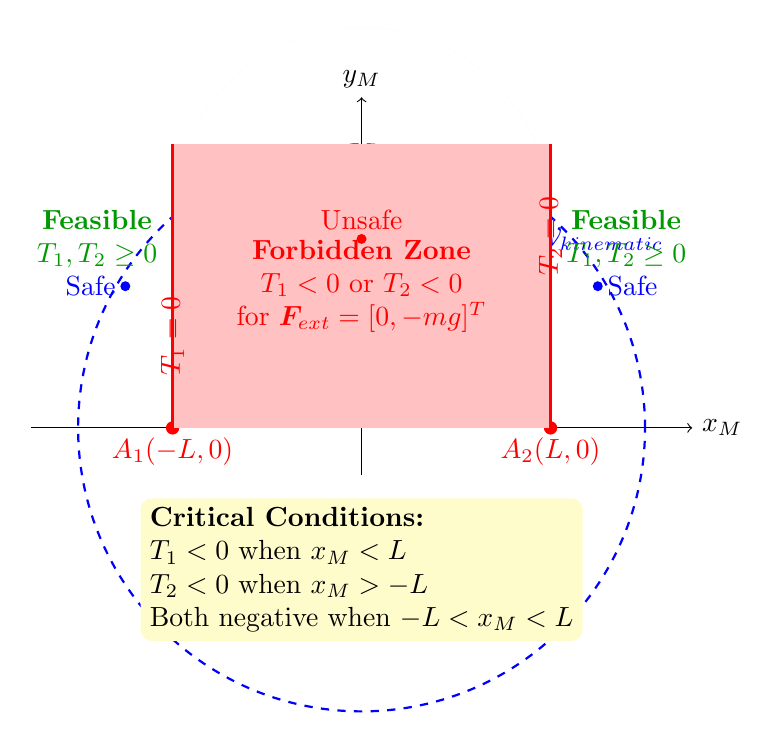
\begin{tikzpicture}[scale=1.2]
    % Coordinate system
    \draw[->] (-3.5,0) -- (3.5,0) node[right] {$x_M$};
    \draw[->] (0,-0.5) -- (0,3.5) node[above] {$y_M$};
    
    % Cable anchor points
    \fill[red] (-2,0) circle (2pt) node[below] {$A_1(-L,0)$};
    \fill[red] (2,0) circle (2pt) node[below] {$A_2(L,0)$};
    
    % Kinematic workspace (circle)
    \draw[thick, blue, dashed] (0,0) circle (3);
    \node[blue] at (2.5,2) {$\mathcal{W}_{kinematic}$};
    
    % Feasible region for downward load (outside forbidden zone)
    \fill[green!20, opacity=0.7] 
        (-2,0) -- (-2,2.236) arc (180:0:2) -- (2,0) -- (2,2.236) arc (0:180:2) -- cycle;
    \fill[white] (-2,0) rectangle (2,3);
    
    % Forbidden zone (between anchors for downward load)
    \fill[red!30, opacity=0.8] (-2,0) rectangle (2,3);
    \node[red, align=center] at (0,1.5) {\textbf{Forbidden Zone} \\ $T_1 < 0$ or $T_2 < 0$ \\ for $\bm{F}_{ext} = [0,-mg]^T$};
    
    % Boundary lines where tensions = 0
    \draw[thick, red] (-2,0) -- (-2,3) node[left, rotate=90, midway] {$T_1 = 0$};
    \draw[thick, red] (2,0) -- (2,3) node[right, rotate=90, midway] {$T_2 = 0$};
    
    % Feasible region annotation
    \node[green!60!black, align=center] at (-2.8,2) {\textbf{Feasible} \\ $T_1, T_2 \geq 0$};
    \node[green!60!black, align=center] at (2.8,2) {\textbf{Feasible} \\ $T_1, T_2 \geq 0$};
    
    % Example end-effector positions
    \fill[blue] (-2.5,1.5) circle (1.5pt) node[left] {Safe};
    \fill[red] (0,2) circle (1.5pt) node[above] {Unsafe};
    \fill[blue] (2.5,1.5) circle (1.5pt) node[right] {Safe};
    
    % Workspace boundary equations
    \node[align=left, fill=yellow!20, rounded corners] at (0,-1.5) {
        \textbf{Critical Conditions:} \\
        $T_1 < 0$ when $x_M < L$ \\
        $T_2 < 0$ when $x_M > -L$ \\
        Both negative when $-L < x_M < L$
    };
\end{tikzpicture}
\caption{Workspace analysis for downward gravitational load. The forbidden zone (red) shows regions where negative cable tensions would be required. The feasible workspace (green) is significantly reduced compared to the kinematic workspace (blue dashed circle).}
\label{fig:workspace_analysis}
\end{figure}

Negative tensions occur when:
\begin{itemize}
    \item $T_1 < 0$: when $x_M < L$ (left side of right anchor)
    \item $T_2 < 0$: when $x_M > -L$ (right side of left anchor)  
    \item Both: when $-L < x_M < L$ (between anchors)
\end{itemize}

This creates a **forbidden zone** between the cable anchors for downward loads.

\subsection{Design and Control Implications}

\subsubsection{Design Optimization}
\textbf{1. Cable Anchor Placement:}
Optimize anchor positions to maximize feasible workspace:
\begin{align}
L_{optimal} &= \arg\max_L |\mathcal{W}_{feasible}(L, \bm{F}_{ext})|
\end{align}

\textbf{2. Link Length Ratios:}
Balance serial chain workspace with cable effectiveness:
\begin{align}
\frac{l_2}{l_1} &= \arg\max_{ratio} |\mathcal{W}_{feasible} \cap \mathcal{W}_{dexterous}|
\end{align}

\textbf{3. Joint Range Limits:}
Coordinate joint limits with cable constraints:
\begin{align}
q_{2,min} &\geq \epsilon > 0 \quad \text{(avoid } q_2 = 0 \text{ singularity)} \\
q_{2,max} &\leq \pi - \epsilon \quad \text{(avoid } q_2 = \pi \text{ singularity)}
\end{align}

\subsubsection{Control Strategies}
\textbf{1. Hybrid Control Architecture:}
Switch between control modes based on tension feasibility:
\begin{algorithm}[H]
\caption{Hybrid Cable-Joint Control}
\begin{algorithmic}
\STATE \textbf{Input:} Desired end-effector position $\bm{x}_{desired}$, external load $\bm{F}_{ext}$
\STATE Compute required cable tensions $T_1, T_2$ from force equilibrium
\IF{$T_1 \geq T_{min}$ AND $T_2 \geq T_{min}$}
    \STATE Use cable control mode
    \STATE Control cable lengths $\rho_1, \rho_2$ to achieve $\bm{x}_{desired}$
\ELSE
    \STATE Use joint control mode
    \STATE Control joint angles $q_1, q_2$ to achieve $\bm{x}_{desired}$
    \STATE Set cable tensions to minimum safe values
\ENDIF
\end{algorithmic}
\end{algorithm}

\textbf{2. Pre-tensioning Strategy:}
Maintain minimum cable tensions to avoid slack and improve responsiveness:
\begin{align}
T_{1,command} &= \max(T_{1,required}, T_{min}) \\
T_{2,command} &= \max(T_{2,required}, T_{min})
\end{align}

Where $T_{min} > 0$ is the minimum safe tension level.

\textbf{3. Workspace Planning:}
Generate trajectories that avoid negative tension regions:
\begin{align}
\bm{x}_{trajectory}(t) &\in \mathcal{W}_{feasible} \quad \forall t \in [0, T_{final}]
\end{align}

\textbf{4. Redundancy Exploitation:}
Use additional degrees of freedom to maintain positive tensions:
\begin{itemize}
    \item Adjust joint configuration while maintaining end-effector position
    \item Vary cable pre-tension levels dynamically
    \item Coordinate multiple cables if available
\end{itemize}

\subsection{Practical Implementation Considerations}

\subsubsection{Sensor Requirements}
\textbf{1. Tension Monitoring:}
\begin{itemize}
    \item Load cells or strain gauges in cable paths
    \item Real-time tension feedback for control
    \item Early warning for approaching negative tension conditions
\end{itemize}

\textbf{2. Position Sensing:}
\begin{itemize}
    \item Joint angle encoders for $q_1, q_2$
    \item Cable length sensors for $\rho_1, \rho_2$
    \item End-effector position confirmation
\end{itemize}

\subsubsection{Safety Considerations}
\textbf{1. Emergency Protocols:}
\begin{itemize}
    \item Automatic joint braking when cable tensions drop
    \item Fail-safe positions with guaranteed positive tensions
    \item Load sharing between joint and cable actuators
\end{itemize}

\textbf{2. Operating Limits:}
\begin{itemize}
    \item Conservative workspace boundaries
    \item Maximum load ratings based on tension analysis
    \item Speed limitations near singular configurations
\end{itemize}

\subsubsection{Computational Requirements}
\textbf{1. Real-time Tension Calculation:}
Fast algorithms for computing required tensions:
\begin{align}
\text{Computation time: } &O(1) \text{ per control cycle} \\
\text{Memory requirement: } &O(1) \text{ for 2D system}
\end{align}

\textbf{2. Workspace Monitoring:}
Efficient methods to check feasibility:
\begin{itemize}
    \item Pre-computed workspace maps
    \item Look-up tables for common load cases
    \item Approximate analytical boundaries
\end{itemize}

\subsection{Summary}
The cable tension constraint analysis reveals that:

\textbf{Key Insights:}
\begin{enumerate}
    \item Cable systems have inherent directional limitations due to tension positivity
    \item Negative tensions create forbidden workspace regions that vary with external loads
    \item Singularities can be triggered by both geometric and force-based conditions
    \item Proper design and control can mitigate but not eliminate these constraints
\end{enumerate}

\textbf{Design Guidelines:}
\begin{enumerate}
    \item Optimize cable anchor placement for maximum feasible workspace
    \item Implement hybrid control strategies to handle tension constraints
    \item Include pre-tensioning systems for improved performance
    \item Plan trajectories considering both kinematic and force constraints
\end{enumerate}

\textbf{Future Research Directions:}
\begin{enumerate}
    \item Optimization of cable arrangements for specific task requirements
    \item Advanced control algorithms that anticipate tension constraints
    \item Integration with machine learning for adaptive workspace planning
    \item Extension to higher-DOF and 3D cable-driven systems
\end{enumerate}

\subsection{Singularity Conditions}

\subsubsection{Determinant-Based Analysis}
For square Jacobians ($n_j + n_c = 3$):
\begin{align}
S(\bm{q}, \bm{\rho}) &= \det(\bm{J}(\bm{q}, \bm{\rho})) \\
&= \det\begin{bmatrix}
\frac{\partial x_M}{\partial q_1} & \frac{\partial x_M}{\partial q_2} \\
\frac{\partial y_M}{\partial q_1} & \frac{\partial y_M}{\partial q_2}
\end{bmatrix} \\
&= l_1 l_2 \sin q_2
\end{align}

Singular configurations satisfy:
\begin{align}
S(\bm{q}, \bm{\rho}) = 0 \quad \Rightarrow \quad q_2 = n\pi, \quad n \in \mathbb{Z}
\end{align}

\subsubsection{SVD-Based Analysis}
Using Singular Value Decomposition:
\begin{align}
\bm{J} &= \bm{U} \bm{\Sigma} \bm{V}^T \\
\sigma_{\min} &= \min(\text{diag}(\bm{\Sigma})) \\
\kappa(\bm{J}) &= \frac{\sigma_{\max}}{\sigma_{\min}}
\end{align}

Singularity conditions:
\begin{align}
\sigma_{\min} &\approx 0 \\
\kappa(\bm{J}) &\to \infty
\end{align}

\subsection{Manipulability Measures}

\subsubsection{Yoshikawa's Manipulability}
\begin{align}
\mu(\bm{q}, \bm{l}) &= \sqrt{\det(\bm{J}\bm{J}^T)} \\
&= \prod_{i=1}^{\text{rank}(\bm{J})} \sigma_i
\end{align}

\subsubsection{Condition Number}
\begin{align}
\kappa(\bm{q}, \bm{l}) &= \|\bm{J}\| \|\bm{J}^{\dagger}\| \\
&= \frac{\sigma_{\max}}{\sigma_{\min}}
\end{align}

where $\bm{J}^{\dagger}$ is the Moore-Penrose pseudoinverse.

\section{Advanced Singularity Analysis}

\subsection{Geometric Interpretation}

\subsubsection{Instantaneous Center of Rotation}
At singular configurations, the instantaneous center of rotation may:
\begin{enumerate}
    \item Move to infinity (pure translation)
    \item Become indeterminate (loss of constraint)
    \item Coincide with special geometric points
\end{enumerate}

\subsubsection{Velocity Space Analysis}
The feasible velocity space is defined by:
\begin{align}
\mathcal{V} &= \{\dot{\bm{x}} : \dot{\bm{x}} = \bm{J}\dot{\bm{q}}, \dot{\bm{q}} \in \mathbb{R}^{n_j+n_c}\}
\end{align}

At singularities, $\dim(\mathcal{V}) < 3$.

\subsection{Bifurcation Analysis}

\subsubsection{Fold Singularities}
Characterized by:
\begin{align}
\det(\bm{J}) &= 0 \\
\nabla(\det(\bm{J})) &\neq \bm{0}
\end{align}

\subsubsection{Cusp Singularities}
Higher-order singularities where:
\begin{align}
\det(\bm{J}) &= 0 \\
\nabla(\det(\bm{J})) &= \bm{0} \\
\nabla^2(\det(\bm{J})) &\neq \bm{0}
\end{align}

\subsection{Dynamic Singularities}

\subsubsection{Acceleration Analysis}
The acceleration equation is:
\begin{align}
\ddot{\bm{x}} &= \bm{J}\ddot{\bm{q}} + \dot{\bm{J}}\dot{\bm{q}} \\
&= \bm{J}\ddot{\bm{q}} + \bm{h}(\bm{q}, \dot{\bm{q}})
\end{align}

Dynamic singularities occur when:
\begin{align}
\bm{h}(\bm{q}, \dot{\bm{q}}) &\notin \text{Range}(\bm{J})
\end{align}

\section{Workspace Analysis}

\subsection{Workspace Classification}

\subsubsection{Primary Workspace}
Points reachable with at least one orientation:
\begin{align}
\mathcal{W}_1 &= \{(x, y) : \exists \theta, \bm{q}, \bm{l} \text{ s.t. } (x, y, \theta) = \bm{f}(\bm{q}, \bm{l})\}
\end{align}

\subsubsection{Secondary Workspace}  
Points reachable with all orientations:
\begin{align}
\mathcal{W}_2 &= \{(x, y) : \forall \theta, \exists \bm{q}, \bm{l} \text{ s.t. } (x, y, \theta) = \bm{f}(\bm{q}, \bm{l})\}
\end{align}

\subsubsection{Dexterous Workspace}
Points where the manipulability is above a threshold:
\begin{align}
\mathcal{W}_d &= \{(x, y) : \mu(\bm{q}, \bm{l}) > \mu_{min}\}
\end{align}

\subsection{Workspace Boundary}
The reachable workspace is bounded by:
\begin{align}
\mathcal{W} &= \{(x, y) : \exists (\bm{q}, \bm{l}) \text{ such that } (x, y) = \bm{f}(\bm{q}, \bm{l})\} \\
\text{subject to: } &\quad \bm{q}_{\min} \leq \bm{q} \leq \bm{q}_{\max} \\
&\quad \bm{l}_{\min} \leq \bm{l} \leq \bm{l}_{\max}
\end{align}

\subsection{Singular Workspace}
The singular workspace is defined as:
\begin{align}
\mathcal{W}_s &= \{(x, y) \in \mathcal{W} : S(\bm{q}, \bm{l}) = 0\}
\end{align}

\section{Computational Methods}

\subsection{Efficient Jacobian Computation}

\subsubsection{Analytical Differentiation}
For computational efficiency, Jacobian elements should be computed analytically:
\begin{align}
J_{ij} &= \frac{\partial f_i}{\partial q_j} \\
&= \sum_{k=j}^{n} \frac{\partial f_i}{\partial T_k} \frac{\partial T_k}{\partial q_j}
\end{align}

\textbf{Cable Angle Derivatives:}
When using $\text{atan2}$ for cable angles, the derivatives are:
\begin{align}
\frac{\partial \alpha_1}{\partial q_i} &= \frac{\partial}{\partial q_i}\text{atan2}(y_M, x_M + L) \\
&= \frac{(x_M + L)\frac{\partial y_M}{\partial q_i} - y_M\frac{\partial x_M}{\partial q_i}}{(x_M + L)^2 + y_M^2} \\
&= \frac{(x_M + L)\frac{\partial y_M}{\partial q_i} - y_M\frac{\partial x_M}{\partial q_i}}{\rho_1^2}
\end{align}

Similarly for $\alpha_2$:
\begin{align}
\frac{\partial \alpha_2}{\partial q_i} &= \frac{(x_M - L)\frac{\partial y_M}{\partial q_i} - y_M\frac{\partial x_M}{\partial q_i}}{\rho_2^2}
\end{align}

These expressions are well-defined for all configurations, unlike the simple $\arctan$ formulation.

\subsubsection{Recursive Computation}
Using the recursive Newton-Euler approach:
\begin{algorithm}
\caption{Recursive Jacobian Computation}
\begin{algorithmic}[1]
\STATE Initialize: $\bm{z}_0 = [0, 0, 1]^T$, $\bm{p}_0 = [0, 0, 0]^T$
\FOR{$i = 1$ to $n$}
    \STATE Compute $\bm{z}_i = \bm{R}_{i-1} \bm{z}_{i-1}$
    \STATE Compute $\bm{p}_i = \bm{p}_{i-1} + \bm{R}_{i-1} \bm{d}_{i-1}$
    \IF{joint $i$ is revolute}
        \STATE $\bm{J}_{v,i} = \bm{z}_{i-1} \times (\bm{p}_n - \bm{p}_{i-1})$
        \STATE $\bm{J}_{\omega,i} = \bm{z}_{i-1}$
    \ELSE
        \STATE $\bm{J}_{v,i} = \bm{z}_{i-1}$
        \STATE $\bm{J}_{\omega,i} = \bm{0}$
    \ENDIF
\ENDFOR
\end{algorithmic}
\end{algorithm}

\subsection{Singularity Detection Algorithms}

\subsubsection{Multi-Method Approach}
\begin{algorithm}
\caption{Comprehensive Singularity Detection}
\begin{algorithmic}[1]
\REQUIRE Configuration $(\bm{q}, \bm{l})$, tolerances $\epsilon_{det}, \epsilon_{svd}, \kappa_{max}$
\ENSURE Singularity status and type
\STATE Compute Jacobian $\bm{J}(\bm{q}, \bm{l})$
\STATE $method1 \leftarrow |\det(\bm{J})| < \epsilon_{det}$
\STATE Compute SVD: $\bm{J} = \bm{U}\bm{\Sigma}\bm{V}^T$
\STATE $\sigma_{min} \leftarrow \min(\text{diag}(\bm{\Sigma}))$
\STATE $method2 \leftarrow \sigma_{min} < \epsilon_{svd}$
\STATE $\kappa \leftarrow \sigma_{max}/\sigma_{min}$
\STATE $method3 \leftarrow \kappa > \kappa_{max}$
\IF{$method1$ OR $method2$ OR $method3$}
    \STATE Classify singularity type
    \RETURN True, singularity\_type
\ELSE
    \RETURN False, None
\ENDIF
\end{algorithmic}
\end{algorithm}

\subsubsection{Adaptive Tolerance Selection}
The tolerances should be adapted based on:
\begin{align}
\epsilon_{det} &= \epsilon_{base} \cdot \|\bm{J}\|_F^{n} \\
\epsilon_{svd} &= \epsilon_{base} \cdot \|\bm{J}\|_2 \\
\kappa_{max} &= \frac{1}{\epsilon_{base}}
\end{align}

Where $\epsilon_{base} = \sqrt{\text{machine precision}}$.

\subsection{Workspace Generation Algorithms}

\subsubsection{Discretization Method}
\begin{algorithm}
\caption{Workspace Boundary Detection}
\begin{algorithmic}[1]
\REQUIRE Grid resolution $\Delta x, \Delta y$, joint limits
\ENSURE Workspace boundary points
\STATE Initialize empty workspace grid
\FOR{$x = x_{min}$ to $x_{max}$ step $\Delta x$}
    \FOR{$y = y_{min}$ to $y_{max}$ step $\Delta y$}
        \STATE solved $\leftarrow$ False
        \FOR{each orientation $\theta$}
            \STATE Try to solve inverse kinematics for $(x, y, \theta)$
            \IF{solution exists within joint limits}
                \STATE Mark $(x, y)$ as reachable
                \STATE Check singularity at solution
                \STATE solved $\leftarrow$ True
                \STATE break
            \ENDIF
        \ENDFOR
        \IF{NOT solved}
            \STATE Mark $(x, y)$ as unreachable
        \ENDIF
    \ENDFOR
\ENDFOR
\STATE Extract boundary from reachable/unreachable interface
\end{algorithmic}
\end{algorithm}

\subsection{Optimization-Based Methods}

\subsubsection{Singularity-Free Path Planning}
Minimize proximity to singularities:
\begin{align}
\min_{\bm{q}(t), \bm{l}(t)} &\quad \int_0^T \left( \frac{1}{\mu(\bm{q}(t), \bm{l}(t))} + \|\dot{\bm{q}}(t)\|^2 + \|\dot{\bm{l}}(t)\|^2 \right) dt \\
\text{s.t.} &\quad \bm{x}(t) = \bm{f}(\bm{q}(t), \bm{l}(t)) \\
&\quad \bm{q}_{min} \leq \bm{q}(t) \leq \bm{q}_{max} \\
&\quad \bm{l}_{min} \leq \bm{l}(t) \leq \bm{l}_{max}
\end{align}

\subsubsection{Singularity Avoidance}
Using null space projection:
\begin{align}
\dot{\bm{q}} &= \bm{J}^{\dagger} \dot{\bm{x}}_{desired} + (\bm{I} - \bm{J}^{\dagger}\bm{J}) \bm{k} \\
\text{where } \bm{k} &= k_0 \nabla_{\bm{q}} \mu(\bm{q}, \bm{l})
\end{align}

\subsection{Workspace Discretization}
For workspace analysis:
\begin{align}
x_i &= x_{\min} + i \Delta x, \quad i = 0, 1, \ldots, N_x \\
y_j &= y_{\min} + j \Delta y, \quad j = 0, 1, \ldots, N_y
\end{align}

\section{Performance Analysis}

\subsection{Computational Complexity}

\subsubsection{Jacobian Computation}
\begin{itemize}
    \item Forward kinematics: $O(n_j)$
    \item Analytical Jacobian: $O(n_j^2 + n_c^2)$  
    \item Numerical Jacobian: $O((n_j + n_c) \cdot \text{FK cost})$
\end{itemize}

\subsubsection{Singularity Detection}
\begin{itemize}
    \item Determinant: $O(n^3)$ where $n = n_j + n_c$
    \item SVD: $O(mn^2)$ where $m = \min(3, n_j + n_c)$
    \item Condition number: Same as SVD
\end{itemize}

\subsubsection{Workspace Generation}
For grid resolution $N_x \times N_y$:
\begin{itemize}
    \item Discretization method: $O(N_x \cdot N_y \cdot \text{IK cost})$
    \item Boundary extraction: $O(N_x \cdot N_y)$
\end{itemize}

\subsection{Accuracy Analysis}

\subsubsection{Numerical Sensitivity}
The sensitivity of singularity detection to numerical errors:
\begin{align}
\frac{d(\det \bm{J})}{d J_{ij}} &= \text{adj}(\bm{J})_{ji} \\
\text{Relative sensitivity: } &\quad \frac{|J_{ij}|}{|\det \bm{J}|} |\text{adj}(\bm{J})_{ji}|
\end{align}

\subsubsection{Condition Number Scaling}
Near singularities, small perturbations cause large changes:
\begin{align}
\|\Delta \dot{\bm{x}}\| &\leq \kappa(\bm{J}) \|\Delta \dot{\bm{q}}\| \\
\text{Amplification factor: } &\quad \kappa(\bm{J}) = \frac{\sigma_{max}}{\sigma_{min}}
\end{align}

\section{Experimental Validation}

\subsection{Hardware Considerations}

\subsubsection{Sensor Requirements}
\begin{itemize}
    \item Joint encoders: Resolution $\geq 2^{12}$ counts/rev
    \item Cable length sensors: Linear encoders or potentiometers
    \item Force/torque sensors: For validation of singularity effects
    \item End-effector pose measurement: Vision system or coordinate measuring machine
\end{itemize}

\subsubsection{Actuator Limitations}
Near singularities, required actuator forces may become infinite:
\begin{align}
\bm{\tau} &= \bm{J}^T \bm{F}_{external} \\
\|\bm{\tau}\| &\leq \frac{\|\bm{F}_{external}\|}{\sigma_{min}(\bm{J})}
\end{align}

\subsection{Validation Protocols}

\subsubsection{Static Singularity Verification}
\begin{enumerate}
    \item Move robot to predicted singular configuration
    \item Apply small end-effector forces in different directions  
    \item Measure resulting joint torques/cable tensions
    \item Verify that some directions require infinite force (within measurement limits)
\end{enumerate}

\subsubsection{Dynamic Response Testing}
\begin{enumerate}
    \item Command motion through singular region
    \item Monitor manipulability index $\mu(t)$
    \item Record maximum joint velocities and accelerations
    \item Verify correlation with predicted singular behavior
\end{enumerate}

\subsection{Benchmark Problems}

\subsubsection{Analytical Test Cases}
Known singular configurations for validation:
\begin{itemize}
    \item Fully extended configuration (boundary singularity)
    \item Folded configuration (interior singularity)  
    \item Cable alignment configurations
    \item Joint limit configurations
\end{itemize}

\section{Validation and Testing}

\subsection{Systematic Test Framework}

\subsubsection{Unit Tests}
Individual component validation:
\begin{itemize}
    \item Forward kinematics accuracy vs. analytical solutions
    \item Jacobian computation vs. numerical differentiation
    \item Singularity detection consistency across methods
    \item Workspace boundary accuracy
\end{itemize}

\subsection{Test Cases}
Comprehensive validation scenarios:

\subsubsection{Known Singular Configurations}
For the specific robot configuration with parameters $l_1 = 1.0$m, $l_2 = 0.8$m, $L = 1.5$m:

\textbf{Serial Chain Singularities:}
\begin{align}
\text{Fully Extended: } &\quad \bm{q}_1 = [0, 0], \quad \bm{p}_M = [1.8, 0] \\
\text{Fully Folded: } &\quad \bm{q}_2 = [0, \pi], \quad \bm{p}_M = [0.2, 0] \\
\text{Vertical Extended: } &\quad \bm{q}_3 = [\pi/2, 0], \quad \bm{p}_M = [0, 1.8] \\
\text{Vertical Folded: } &\quad \bm{q}_4 = [\pi/2, \pi], \quad \bm{p}_M = [0, 0.2]
\end{align}

\textbf{Cable Singularities:}
\begin{align}
\text{X-axis alignment: } &\quad y_M = 0 \text{ (any configuration on X-axis)} \\
\text{Y-axis symmetry: } &\quad x_M = 0 \text{ (configurations on Y-axis)} \\
\text{Anchor point proximity: } &\quad \bm{p}_M \approx (-L, 0) \text{ or } (L, 0)
\end{align}

\textbf{Combined Singularities:}
\begin{align}
\text{Origin vicinity: } &\quad \bm{q} = [\pi/2, \pi], \quad \bm{p}_M = [0, 0.2] \\
\text{Boundary singularity: } &\quad \bm{q} = [0, 0], \quad \bm{p}_M = [1.8, 0]
\end{align}

\subsubsection{Boundary Conditions}
Test configurations at workspace boundaries and joint limits.

\subsection{Numerical Tolerances}
\begin{align}
\epsilon_{det} &= 10^{-6} \quad \text{(determinant tolerance)} \\
\epsilon_{svd} &= 10^{-8} \quad \text{(SVD tolerance)} \\
\kappa_{max} &= 10^{6} \quad \text{(maximum condition number)}
\end{align}

\section{Practical Implementation Considerations}

\subsection{Real-Time Implementation}

\subsubsection{Computational Optimization}
For real-time control (typical requirements: $f > 1$ kHz):
\begin{itemize}
    \item Pre-compute workspace singularity map offline
    \item Use lookup tables for dense grid regions
    \item Implement fast approximation methods for online queries
    \item Utilize parallel computation for Jacobian elements
\end{itemize}

\subsubsection{Memory Management}
\begin{align}
\text{Workspace map size: } &\quad N_x \times N_y \times N_\theta \times \text{sizeof(float)} \\
\text{Typical example: } &\quad 100 \times 100 \times 36 \times 4 = 1.44 \text{ MB}
\end{align}

\subsection{Error Propagation Analysis}

\subsubsection{Parameter Uncertainties}
Effect of kinematic parameter errors on singularity detection:
\begin{align}
\Delta(\det \bm{J}) &= \sum_{i} \frac{\partial(\det \bm{J})}{\partial p_i} \Delta p_i \\
\text{where } p_i &\in \{L_1, L_2, \ldots, r_1, r_2, \ldots\}
\end{align}

\subsubsection{Measurement Noise}
Joint angle measurement errors propagate as:
\begin{align}
\bm{\Sigma}_J &= \sum_{i=1}^{n_j} \left(\frac{\partial \bm{J}}{\partial q_i}\right) \sigma_{q_i}^2 \left(\frac{\partial \bm{J}}{\partial q_i}\right)^T
\end{align}

\subsection{Safety Considerations}

\subsubsection{Singularity Avoidance Zones}
Define safety margins around singular configurations:
\begin{align}
\text{Warning zone: } &\quad \mu(\bm{q}, \bm{l}) < \mu_{warn} \\
\text{Forbidden zone: } &\quad \mu(\bm{q}, \bm{l}) < \mu_{stop}
\end{align}

Typical values: $\mu_{warn} = 0.1$, $\mu_{stop} = 0.01$.

\subsubsection{Emergency Procedures}
When approaching singularities:
\begin{enumerate}
    \item Reduce motion speed proportionally to $\mu^{-1}$
    \item Activate redundancy resolution
    \item Switch to alternative control strategies
    \item Emergency stop if no solution exists
\end{enumerate}

\section{Software Architecture}

\subsection{Class Hierarchy}
Suggested object-oriented implementation:
\begin{verbatim}
class Robot:
    - parameters: RobotParameters
    - forward_kinematics(): pose
    - inverse_kinematics(): joint_config
    
class Jacobian:
    - robot: Robot  
    - compute_jacobian(): matrix
    - compute_reduced_jacobian(): matrix
    
class SingularityAnalyzer:
    - jacobian: Jacobian
    - detect_singularity(): bool, type
    - compute_manipulability(): float
    - compute_condition_number(): float
    
class WorkspaceAnalyzer:
    - robot: Robot
    - analyzer: SingularityAnalyzer
    - generate_workspace(): workspace_map
    - plot_singularities(): visualization
\end{verbatim}

\subsection{Configuration Management}
Use JSON/YAML for parameter specification:
\begin{verbatim}
{
  "serial_chain": {
    "n_joints": 2,
    "link_lengths": [1.0, 0.8],
    "joint_limits": [[-pi, pi], [-pi, pi]]
  },
  "cables": {
    "n_cables": 2,
    "anchor_points": [[-1.5, 0.0], [1.5, 0.0]],
    "length_limits": [[0.5, 3.0], [0.5, 3.0]]
  },
  "analysis": {
    "tolerances": {
      "determinant": 1e-6,
      "svd": 1e-8,
      "condition_max": 1e6
    },
    "use_atan2": true
  }
}
\end{verbatim}

\subsection{Implementation Notes for atan2}
\begin{itemize}
    \item Use \texttt{numpy.arctan2(y, x)} in Python implementation
    \item Always pass arguments in correct order: \texttt{atan2(y, x)}
    \item Handle numerical precision near singular points
    \item Consider angle wrapping for continuous trajectories
    \item Use \texttt{math.atan2()} for scalar operations
\end{itemize}

\textbf{Example Python Implementation:}
\begin{verbatim}
import numpy as np

def cable_angles(x_M, y_M, L):
    """Compute cable angles using atan2"""
    alpha_1 = np.arctan2(y_M, x_M + L)
    alpha_2 = np.arctan2(y_M, x_M - L)
    return alpha_1, alpha_2

def cable_angle_derivatives(x_M, y_M, dx_dq, dy_dq, L):
    """Compute derivatives of cable angles w.r.t joint variables"""
    rho_1_sq = (x_M + L)**2 + y_M**2
    rho_2_sq = (x_M - L)**2 + y_M**2
    
    dalpha1_dq = ((x_M + L) * dy_dq - y_M * dx_dq) / rho_1_sq
    dalpha2_dq = ((x_M - L) * dy_dq - y_M * dx_dq) / rho_2_sq
    
    return dalpha1_dq, dalpha2_dq
\end{verbatim}

\section{References and Further Reading}

\subsection{Primary References}
\begin{enumerate}
\item Original paper: AJEASSP 2022, pages 197-208
\item Gosselin, C., Angeles, J.: "Singularity analysis of closed-loop kinematic chains", IEEE Trans. Robotics and Automation, 1990
\item Ma, O., Angeles, J.: "Architecture singularities of platform manipulators", IEEE Int. Conf. Robotics and Automation, 1991
\item Merlet, J.P.: "Parallel Robots", Springer, 2006
\item Salisbury, J.K., Craig, J.J.: "Articulated hands: Force control and kinematic issues", Int. J. Robotics Research, 1982
\end{enumerate}

\subsection{Supplementary References}
\begin{enumerate}
\item Spong, M.W., Hutchinson, S., Vidyasagar, M.: "Robot Modeling and Control", Wiley, 2020
\item Craig, J.J.: "Introduction to Robotics: Mechanics and Control", Pearson, 2017
\item Lynch, K.M., Park, F.C.: "Modern Robotics", Cambridge University Press, 2017
\item Siciliano, B., Khatib, O.: "Springer Handbook of Robotics", Springer, 2016
\end{enumerate}

\subsection{Cable-Driven Robot Specific}
\begin{enumerate}
\item Kawamura, S., et al.: "Development of an ultrahigh speed robot FALCON using wire drive system", IEEE Int. Conf. Robotics and Automation, 1995
\item Albus, J., et al.: "The NIST robocrane", J. Robotic Systems, 1993
\item Verhoeven, R.: "Analysis of the workspace of tendon-based Stewart platforms", PhD thesis, University of Duisburg-Essen, 2004
\end{enumerate}

\appendix
\section{Notation and Symbol Reference}

This appendix provides a comprehensive reference for all mathematical symbols, variables, and notation used throughout this document. This standardized notation ensures consistency and eliminates ambiguity in mathematical derivations and implementation.

\subsection{Robot Geometry and Configuration}

\begin{table}[h!]
\centering
\caption{Robot Geometric Parameters}
\begin{tabular}{|c|l|c|l|}
\hline
\textbf{Symbol} & \textbf{Description} & \textbf{Units} & \textbf{Type} \\
\hline
$l_1$ & Length of first link (base to elbow) & m & Fixed parameter \\
$l_2$ & Length of second link (elbow to end-effector) & m & Fixed parameter \\
$L$ & Half-distance between cable anchor points & m & Fixed parameter \\
$q_1$ & First joint angle (base joint) & rad & Variable \\
$q_2$ & Second joint angle (elbow joint) & rad & Variable \\
$\bm{q}$ & Joint angle vector $[q_1, q_2]^T$ & rad & Vector variable \\
\hline
\end{tabular}
\end{table}

\subsection{Cable System Parameters}

\begin{table}[h!]
\centering
\caption{Cable System Notation}
\begin{tabular}{|c|l|c|l|}
\hline
\textbf{Symbol} & \textbf{Description} & \textbf{Units} & \textbf{Type} \\
\hline
$\rho_1$ & Left cable length (variable, motor-controlled) & m & Control input \\
$\rho_2$ & Right cable length (variable, motor-controlled) & m & Control input \\
$\bm{\rho}$ & Cable length vector $[\rho_1, \rho_2]^T$ & m & Vector variable \\
$\alpha_1$ & Left cable angle (from horizontal) & rad & Computed variable \\
$\alpha_2$ & Right cable angle (from horizontal) & rad & Computed variable \\
$T_1$ & Left cable tension force & N & Control input \\
$T_2$ & Right cable tension force & N & Control input \\
$\bm{T}$ & Cable tension vector $[T_1, T_2]^T$ & N & Vector variable \\
\hline
\multicolumn{4}{|l|}{\textbf{Cable Tension Constraints:}} \\
\hline
$T_1 \geq 0$ & Non-negative left cable tension constraint & - & Physical constraint \\
$T_2 \geq 0$ & Non-negative right cable tension constraint & - & Physical constraint \\
\hline
\end{tabular}
\end{table}

\subsection{Coordinate Frames and Positions}

\begin{table}[h!]
\centering
\caption{Coordinate System Notation}
\begin{tabular}{|c|l|c|l|}
\hline
\textbf{Symbol} & \textbf{Description} & \textbf{Units} & \textbf{Type} \\
\hline
$\{0\}$ & Base coordinate frame (world frame) & - & Fixed frame \\
$\{1\}$ & First joint coordinate frame & - & Moving frame \\
$\{2\}$ & End-effector coordinate frame & - & Moving frame \\
$O$ & Origin of base frame (joint 1 center) & - & Fixed point \\
$A$ & Elbow joint center (joint 2 center) & - & Moving point \\
$M$ & End-effector point (cable attachment) & - & Moving point \\
$x_M, y_M$ & End-effector position coordinates & m & Computed variables \\
$\bm{p}_M$ & End-effector position vector $[x_M, y_M]^T$ & m & Vector variable \\
\hline
\end{tabular}
\end{table}

\subsection{Cable Anchor Points and Geometry}

\begin{table}[h!]
\centering
\caption{Cable Anchor Point Notation}
\begin{tabular}{|c|l|c|l|}
\hline
\textbf{Symbol} & \textbf{Description} & \textbf{Units} & \textbf{Type} \\
\hline
$A_1$ & Left cable anchor point position & - & Fixed point \\
$A_2$ & Right cable anchor point position & - & Fixed point \\
$\bm{A}_1$ & Left anchor position vector $[-L, 0]^T$ & m & Fixed vector \\
$\bm{A}_2$ & Right anchor position vector $[L, 0]^T$ & m & Fixed vector \\
$\bm{u}_1$ & Left cable unit direction vector & - & Computed vector \\
$\bm{u}_2$ & Right cable unit direction vector & - & Computed vector \\
\hline
\end{tabular}
\end{table}

\subsection{Denavit-Hartenberg Parameters}

\begin{table}[h!]
\centering
\caption{DH Parameter Notation (Distinct from Cable Angles)}
\begin{tabular}{|c|l|c|l|}
\hline
\textbf{Symbol} & \textbf{Description} & \textbf{Units} & \textbf{Type} \\
\hline
$a_i$ & Link length (DH parameter) & m & Fixed parameter \\
$\alpha_{DH,i}$ & Link twist angle (DH parameter) & rad & Fixed parameter \\
$d_i$ & Link offset (DH parameter) & m & Fixed parameter \\
$\theta_i$ & Joint angle (DH parameter) & rad & Variable \\
\hline
\multicolumn{4}{|l|}{\textbf{Specific Values for 2-DOF Planar Robot:}} \\
\hline
$a_1 = l_1$ & First link length & m & $a_1 = l_1$ \\
$a_2 = l_2$ & Second link length & m & $a_2 = l_2$ \\
$\alpha_{DH,1} = 0$ & First link twist (planar motion) & rad & 0 \\
$\alpha_{DH,2} = 0$ & Second link twist (planar motion) & rad & 0 \\
$d_1 = 0$ & First joint offset (revolute joint) & m & 0 \\
$d_2 = 0$ & Second joint offset (revolute joint) & m & 0 \\
$\theta_1 = q_1$ & First joint variable & rad & Variable \\
$\theta_2 = q_2$ & Second joint variable & rad & Variable \\
\hline
\end{tabular}
\end{table}

\subsection{Transformation Matrices}

\begin{table}[h!]
\centering
\caption{Transformation Matrix Notation}
\begin{tabular}{|c|l|c|l|}
\hline
\textbf{Symbol} & \textbf{Description} & \textbf{Dimensions} & \textbf{Meaning} \\
\hline
$\bm{T}_j^i$ & Transform from frame $\{i\}$ to frame $\{j\}$ & $3 \times 3$ & Homogeneous transform \\
$\bm{T}_1^0$ & Base to first joint transformation & $3 \times 3$ & Fixed to moving \\
$\bm{T}_2^1$ & First to second joint transformation & $3 \times 3$ & Moving to moving \\
$\bm{T}_2^0$ & Base to end-effector transformation & $3 \times 3$ & Complete chain \\
$\bm{R}_j^i$ & Rotation matrix from frame $\{i\}$ to $\{j\}$ & $2 \times 2$ & Rotation only \\
$\bm{p}_j^i$ & Position vector of frame $\{j\}$ in frame $\{i\}$ & $2 \times 1$ & Translation only \\
\hline
\end{tabular}
\end{table}

\subsection{Kinematics and Dynamics}

\begin{table}[h!]
\centering
\caption{Kinematic and Dynamic Variables}
\begin{tabular}{|c|l|c|l|}
\hline
\textbf{Symbol} & \textbf{Description} & \textbf{Units} & \textbf{Type} \\
\hline
$\dot{q}_1, \dot{q}_2$ & Joint angular velocities & rad/s & Time derivatives \\
$\dot{\bm{q}}$ & Joint velocity vector $[\dot{q}_1, \dot{q}_2]^T$ & rad/s & Vector variable \\
$\dot{\rho}_1, \dot{\rho}_2$ & Cable length change rates & m/s & Time derivatives \\
$\dot{\bm{\rho}}$ & Cable velocity vector $[\dot{\rho}_1, \dot{\rho}_2]^T$ & m/s & Vector variable \\
$\dot{x}_M, \dot{y}_M$ & End-effector velocity components & m/s & Computed variables \\
$\dot{\bm{x}}$ & End-effector velocity vector $[\dot{x}_M, \dot{y}_M]^T$ & m/s & Vector variable \\
$\tau_1, \tau_2$ & Joint torques (if used) & N$\cdot$m & Control inputs \\
$\bm{\tau}$ & Joint torque vector (if used) & N$\cdot$m & Vector variable \\
\hline
\end{tabular}
\end{table}

\subsection{Jacobian Matrices}

\begin{table}[h!]
\centering
\caption{Jacobian Matrix Notation}
\begin{tabular}{|c|l|c|l|}
\hline
\textbf{Symbol} & \textbf{Description} & \textbf{Dimensions} & \textbf{Physical Meaning} \\
\hline
$\bm{J}_q$ & Serial joint Jacobian & $2 \times 2$ & $\frac{\partial \bm{x}}{\partial \bm{q}}$ \\
$\bm{J}_{\rho}$ & Cable Jacobian & $2 \times 2$ & $\frac{\partial \bm{x}}{\partial \bm{\rho}}$ \\
$\bm{J}$ & Complete system Jacobian & $2 \times 4$ & $[\bm{J}_q \quad \bm{J}_{\rho}]$ \\
$\bm{J}_{red}$ & Reduced Jacobian (constrained system) & $2 \times 2$ & Effective joint-space Jacobian \\
\hline
\end{tabular}
\end{table}

\subsection{Constraint Equations}

\begin{table}[h!]
\centering
\caption{Constraint Equation Notation}
\begin{tabular}{|c|l|c|l|}
\hline
\textbf{Symbol} & \textbf{Description} & \textbf{Dimensions} & \textbf{Type} \\
\hline
$g_1(\bm{q}, \rho_1)$ & Left cable geometric constraint & scalar & Nonlinear function \\
$g_2(\bm{q}, \rho_2)$ & Right cable geometric constraint & scalar & Nonlinear function \\
$\bm{g}(\bm{q}, \bm{\rho})$ & Constraint vector $[g_1, g_2]^T$ & $2 \times 1$ & Vector function \\
$\bm{G}_q$ & Constraint Jacobian w.r.t. joints & $2 \times 2$ & $\frac{\partial \bm{g}}{\partial \bm{q}}$ \\
$\bm{G}_{\rho}$ & Constraint Jacobian w.r.t. cables & $2 \times 2$ & $\frac{\partial \bm{g}}{\partial \bm{\rho}}$ \\
\hline
\end{tabular}
\end{table}

\subsection{Forces and Unit Vectors}

\begin{table}[h!]
\centering
\caption{Force and Direction Vectors}
\begin{tabular}{|c|l|c|l|}
\hline
\textbf{Symbol} & \textbf{Description} & \textbf{Units} & \textbf{Type} \\
\hline
$\bm{F}_1$ & Left cable force vector & N & Force vector \\
$\bm{F}_2$ & Right cable force vector & N & Force vector \\
$\bm{F}_{cable}$ & Total cable force $\bm{F}_1 + \bm{F}_2$ & N & Resultant force \\
$\bm{F}_{ext}$ & External force at end-effector & N & Applied load \\
$F_{ext,x}, F_{ext,y}$ & External force components & N & Force components \\
$P_1, P_2$ & Gravitational forces at centers of mass & N & Force magnitudes \\
$G_1, G_2$ & Centers of mass of links 1 and 2 & - & Points \\
\hline
\end{tabular}
\end{table}

\subsection{Mathematical Functions and Operators}

\begin{table}[h!]
\centering
\caption{Mathematical Operations and Functions}
\begin{tabular}{|c|l|c|l|}
\hline
\textbf{Symbol} & \textbf{Description} & \textbf{Domain/Range} & \textbf{Notes} \\
\hline
$\text{atan2}(y,x)$ & Four-quadrant arctangent function & $(-\pi, \pi]$ & Robust angle calculation \\
$\|\bm{v}\|$ & Euclidean norm of vector $\bm{v}$ & $[0, \infty)$ & Vector magnitude \\
$\det(\bm{A})$ & Determinant of matrix $\bm{A}$ & $\mathbb{R}$ & Scalar value \\
$\bm{A}^{-1}$ & Matrix inverse of $\bm{A}$ & Same size as $\bm{A}$ & When $\det(\bm{A}) \neq 0$ \\
$\bm{A}^T$ & Matrix transpose of $\bm{A}$ & Transposed dimensions & Row-column exchange \\
$\frac{\partial f}{\partial x}$ & Partial derivative of $f$ w.r.t. $x$ & Varies & Rate of change \\
\hline
\end{tabular}
\end{table}

\subsection{Singularity Analysis Notation}

\begin{table}[h!]
\centering
\caption{Singularity Analysis Symbols}
\begin{tabular}{|c|l|c|l|}
\hline
\textbf{Symbol} & \textbf{Description} & \textbf{Condition} & \textbf{Physical Meaning} \\
\hline
Type I & Serial chain singularity & $\det(\bm{J}_q) = 0$ & Loss of joint DOF \\
Type II & Cable singularity & $\det(\bm{G}_{\rho}) = 0$ & Cable constraints dependent \\
Type III & Combined singularity & $\det(\bm{J}_{red}) = 0$ & System-level singularity \\
$q_2 = 0$ & Fully extended configuration & $\sin(q_2) = 0$ & Serial arm straight \\
$q_2 = \pi$ & Fully folded configuration & $\sin(q_2) = 0$ & Serial arm folded back \\
\hline
\end{tabular}
\end{table}

\subsection{Important Relationships and Formulas}

\begin{table}[h!]
\centering
\caption{Key Mathematical Relationships}
\begin{tabular}{|c|l|}
\hline
\textbf{Category} & \textbf{Formula} \\
\hline
\multirow{4}{*}{Forward Kinematics} & $x_M = l_1\cos q_1 + l_2\cos(q_1 + q_2)$ \\
& $y_M = l_1\sin q_1 + l_2\sin(q_1 + q_2)$ \\
& $\rho_1 = \sqrt{(x_M + L)^2 + y_M^2}$ \\
& $\rho_2 = \sqrt{(x_M - L)^2 + y_M^2}$ \\
\hline
\multirow{2}{*}{Cable Angles} & $\alpha_1 = \text{atan2}(y_M, x_M + L)$ \\
& $\alpha_2 = \text{atan2}(y_M, x_M - L)$ \\
\hline
\multirow{2}{*}{Cable Unit Vectors} & $\bm{u}_1 = \frac{1}{\rho_1}[x_M + L, y_M]^T$ \\
& $\bm{u}_2 = \frac{1}{\rho_2}[x_M - L, y_M]^T$ \\
\hline
\multirow{2}{*}{Velocity Kinematics} & $\dot{\bm{x}} = \bm{J}_q \dot{\bm{q}} + \bm{J}_{\rho} \dot{\bm{\rho}}$ \\
& $\dot{\bm{x}} = \bm{J}_{red} \dot{\bm{q}}$ (constrained) \\
\hline
Singularity Conditions & $\det(\bm{J}_q) = l_1 l_2 \sin q_2 = 0$ \\
\hline
\multirow{3}{*}{Cable Tension Constraints} & $T_1 \geq 0, T_2 \geq 0$ (Non-negative tensions) \\
& $\sin(\alpha_2 - \alpha_1) \neq 0$ (Non-parallel cables) \\
& Force equilibrium: $T_1 \bm{u}_1 + T_2 \bm{u}_2 + \bm{F}_{ext} = \bm{0}$ \\
\hline
\end{tabular}
\end{table}

\subsection{Workspace Definitions}

\begin{table}[h!]
\centering
\caption{Workspace and Constraint Set Notation}
\begin{tabular}{|c|l|}
\hline
\textbf{Symbol} & \textbf{Description} \\
\hline
$\mathcal{W}_{kinematic}$ & Kinematic workspace (reachable by serial chain) \\
$\mathcal{W}_{feasible}$ & Feasible workspace (positive cable tensions) \\
$\mathcal{W}_{cable-limited}$ & Cable-limited regions (negative tensions required) \\
$\mathcal{W}_{singular}$ & Singular configurations ($\det(\bm{J}) = 0$) \\
\hline
\multicolumn{2}{|l|}{\textbf{Mathematical Definitions:}} \\
\hline
$\mathcal{W}_{kinematic}$ & $\{(x_M, y_M) : x_M^2 + y_M^2 \leq (l_1 + l_2)^2\}$ \\
$\mathcal{W}_{feasible}$ & $\{(x_M, y_M) : T_1 \geq 0 \text{ and } T_2 \geq 0\}$ \\
$\mathcal{W}_{cable-limited}$ & $\{(x_M, y_M) : T_1 < 0 \text{ or } T_2 < 0\}$ \\
$\mathcal{W}_{singular}$ & $\{(x_M, y_M) : q_2 = n\pi, n \in \mathbb{Z}\}$ \\
\hline
\end{tabular}
\end{table}

\subsection{Notation Conventions}

\begin{itemize}
    \item \textbf{Scalars}: Regular italic font (e.g., $q_1$, $l_1$, $\rho_1$)
    \item \textbf{Vectors}: Bold lowercase (e.g., $\bm{q}$, $\bm{p}_M$, $\bm{u}_1$)
    \item \textbf{Matrices}: Bold uppercase (e.g., $\bm{T}_1^0$, $\bm{J}_q$, $\bm{R}$)
    \item \textbf{Frames}: Curly braces (e.g., $\{0\}$, $\{1\}$, $\{2\}$)
    \item \textbf{Points}: Regular uppercase (e.g., $O$, $A$, $M$, $A_1$, $A_2$)
    \item \textbf{Subscripts}: Parameter index or frame reference
    \item \textbf{Superscripts}: Reference frame for transformations
    \item \textbf{Dots}: Time derivatives (e.g., $\dot{q}_1$, $\dot{\bm{x}}$)
\end{itemize}

\subsection{Critical Distinctions}

\begin{table}[h!]
\centering
\caption{Commonly Confused Notation - Key Distinctions}
\begin{tabular}{|c|c|l|}
\hline
\textbf{Symbol} & \textbf{NOT} & \textbf{Distinction} \\
\hline
$l_1, l_2$ & $\rho_1, \rho_2$ & Link lengths (fixed) vs Cable lengths (variable) \\
$\alpha_1, \alpha_2$ & $\alpha_{DH,1}, \alpha_{DH,2}$ & Cable angles vs DH twist parameters \\
$T_1, T_2$ & $\tau_1, \tau_2$ & Cable tensions vs Joint torques \\
$\bm{J}_{\rho}$ & $\bm{J}_l$ & Cable Jacobian (corrected notation) \\
$\bm{G}_{\rho}$ & $\bm{G}_l$ & Constraint Jacobian (corrected notation) \\
\hline
\end{tabular}
\end{table}

\section{Derivation Details}
% TODO: Add detailed mathematical derivations

\section{Code Implementation Notes}
% TODO: Add implementation-specific notes and algorithms

\end{document}